% ======================== main.tex ========================
% ----------------------------------------------------------

\documentclass[12pt,a4paper,oneside]{book}

% =============================
% =============================
\usepackage{fontspec}
\IfFontExistsTF{Times New Roman}{\setmainfont{Times New Roman}}{\setmainfont{Tinos}}
\setmonofont{DejaVu Sans Mono}[Scale=0.80]

% =============================
% =============================
\usepackage{amsmath}
\usepackage{amssymb}
\usepackage{amsthm}
\usepackage{bm}
\usepackage{mathrsfs}
\usepackage{mathtools}

% =============================
% =============================
\usepackage{geometry}
\usepackage{setspace}
\usepackage{graphicx}
\usepackage{caption}
\usepackage{subcaption}
\usepackage{placeins}
\usepackage{booktabs}
\usepackage{enumitem}
\usepackage[bottom]{footmisc}
\usepackage{fancyhdr}

% =============================
% =============================
\usepackage[dvipsnames, svgnames]{xcolor}
\usepackage{pifont}
\usepackage{tcolorbox}
\tcbuselibrary{skins,breakable}

% =============================
% =============================
\usepackage{listings}
\usepackage{algorithm}
\usepackage[noend]{algpseudocode}
\usepackage{etoolbox}

% =============================
% =============================
\usepackage{ifthen}
\usepackage{hyperref}
\usepackage[backend=biber,style=alphabetic,sorting=nyt]{biblatex}
\addbibresource{ref.bib}
\AtBeginBibliography{\sloppy}
\usepackage{url}
\usepackage{float}
\usepackage{appendix}
\usepackage{animate}
\usepackage{tikz}

% =============================
% =============================
\definecolor{greenshade}{rgb}{0.9, 1, 0.9}
\definecolor{green}{rgb}{0.2, 0.6, 0.2}
\definecolor{axmBack}{rgb}{0.95, 0.95, 1}
\definecolor{axmFrame}{rgb}{0.5, 0.5, 1}
\definecolor{axmTitle}{rgb}{0.2, 0.2, 0.6}
\definecolor{lightblue}{rgb}{0.8, 0.9, 1}
\definecolor{lightgray}{rgb}{0.95, 0.95, 0.95}
\definecolor{lightyellow}{rgb}{1, 0.98, 0.9}
\definecolor{lightcyan}{rgb}{0.9, 1, 1}
\definecolor{SkyBlue}{rgb}{0.2,0.6,1}
\definecolor{lightcyanq}{RGB}{220, 245, 240}

\newtheoremstyle{mythm}
  {\topsep}{\topsep}{\itshape}{}{\bfseries}{.}{.5em}{}
\theoremstyle{mythm}
\newtheorem{theorem}{Theorem}[chapter]
\newtheorem{lemma}[theorem]{Lemma}
\newtheorem{corollary}[theorem]{Corollary}
\newtheorem{proposition}[theorem]{Proposition}
\newtheorem{axiom}{Axiom}[chapter]

\newtheoremstyle{mydef}
  {\topsep}{\topsep}{\upshape}{}{\bfseries}{.}{.5em}{}
\theoremstyle{mydef}
\newtheorem{definition}{Definition}[chapter]
\newtheorem{example}{Example}[chapter]
\newtheorem{remark}{Remark}[chapter]

\renewenvironment{proof}{\indent\textcolor{SkyBlue}{\textbf{Proof.}}\;}{\qed\par}
\newenvironment{solution}{\indent\textcolor{SkyBlue}{\textbf{Solution.}}\;}{\qed\par}

\newtcolorbox[auto counter, number within=chapter, list inside=mydefbox]{defn}[1][]{
  enhanced, breakable,
  colback=greenshade, colframe=green, arc=3mm,
  title={\textbf{Definition \thetcbcounter\ #1}},
  coltitle=black, fonttitle=\bfseries
}

\newtcolorbox[auto counter, number within=chapter]{axiombox}[1][]{
  enhanced, breakable,
  colback=axmBack, colframe=axmFrame, arc=3mm,
  title={\textbf{Axiom \thetcbcounter\ #1}},
  coltitle=axmTitle, fonttitle=\bfseries,
}

\newtcolorbox{Notice}[1][Notice]{
  colback=lightblue, colframe=black, arc=3mm,
  title={\textbf{#1}}, coltitle=white, fonttitle=\bfseries
}

\newtcolorbox{Proof}{
  colback=lightgray, colframe=black, arc=3mm,
  title={\textbf{Proof}}, coltitle=black, fonttitle=\bfseries
}

\newtcolorbox{Derivation}[1][]{
  enhanced, breakable,
  colback=lightyellow, colframe=black, arc=3mm,
  title={\textbf{Derivation}}, coltitle=white, fonttitle=\bfseries,
  boxsep=2mm, #1
}

\newtcolorbox{examplebox}[1][Example]{
  colback=lightcyan, colframe=black, arc=3mm,
  title={\textbf{#1}}, coltitle=black, fonttitle=\bfseries
}

\newtcolorbox{Question}[1][]{
  enhanced, breakable, colback=lightcyanq, colframe=black, arc=3mm,
  title={\textbf{Question}}, coltitle=white, fonttitle=\bfseries, boxsep=2mm, #1
}

% =============================
% =============================
\definecolor{codebg}{RGB}{245,245,245}
\definecolor{codeframe}{RGB}{220,220,220}

\lstset{
  basicstyle=\small\ttfamily,
  backgroundcolor=\color{codebg},
  frame=single,
  framesep=5pt,
  rulecolor=\color{codeframe},
  framerule=0.8pt,
  numbers=left,
  numberstyle=\footnotesize\color{gray},
  numbersep=5pt,
  stepnumber=1,
  firstnumber=1,
  tabsize=4,
  showspaces=false,
  showstringspaces=false,
  showtabs=false,
  breaklines=true,
  breakatwhitespace=false,
  prebreak=\raisebox{0ex}[0ex][0ex]{\ensuremath{\hookleftarrow}},
  keywordstyle=\color[RGB]{0,0,255}\bfseries,
  commentstyle=\color[RGB]{34,139,34}\itshape,
  stringstyle=\color[RGB]{178,34,34},
  identifierstyle=\color{black},
  captionpos=b,
  xleftmargin=15pt,
  xrightmargin=5pt,
  keepspaces=true,
  aboveskip=1em,
  belowskip=1em
}

\lstdefinelanguage{Python}{
  keywords={False,None,True,and,as,assert,async,await,break,class,continue,def,
            del,elif,else,except,finally,for,from,global,if,import,in,is,lambda,
            nonlocal,not,or,pass,raise,return,try,while,with,yield},
  keywords=[2]{self,cls,__init__,__name__,__main__},
  keywords=[3]{print,input,len,str,int,float,list,dict,set,tuple,range},
  sensitive=true,
  comment=[l]{\#},
  morecomment=[s]{"""}{"""},
  morecomment=[s]{'''}{'''},
  string=[b]',
  string=[b]",
  morestring=[s]{r'}{'},
  morestring=[s]{r"}{"}
}

\lstdefinelanguage{Matlab}{
  keywords={break,case,catch,classdef,continue,else,elseif,end,for,function,
            global,if,otherwise,parfor,persistent,return,spmd,switch,try,while},
  keywords=[2]{pi,eps,inf,nan,ans},
  keywords=[3]{plot,sin,cos,exp,log,mean,std},
  sensitive=false,
  comment=[l]{\%},
  morecomment=[s]{\%\{}{\%\}},
  string=[b]',
  string=[b]"
}

\lstdefinelanguage{C}{
  keywords={auto,break,case,char,const,continue,default,do,double,else,enum,
            extern,float,for,goto,if,inline,int,long,register,restrict,return,
            short,signed,sizeof,static,struct,switch,typedef,union,unsigned,
            void,volatile,while,_Bool,_Complex,_Imaginary},
  sensitive=true,
  morecomment=[l]{//},
  morecomment=[s]{/*}{*/},
  string=[b]',
  string=[b]",
  alsoletter=\#,
  morekeywords=[2]{printf,scanf,malloc,free,sizeof}
}

\lstdefinelanguage{Mathematica}{
  keywords={If,Do,For,While,Module,Block,With,Catch,Throw,Return,Break,Continue,
            Function,Pattern,Set,SetDelayed,Rule,RuleDelayed,ReplaceAll,
            ReplaceRepeated,True,False,Null,List,Table,Map,Apply,Flatten},
  morekeywords=[2]{Sin,Cos,Log,Integrate,D,Plot,Solve,Expand},
  sensitive=true,
  comment=[l]{(*)},
  morecomment=[l]{*)},
  string=[b]",
  alsoletter={@,?,\#},
  morestring=[b]`
}

\lstdefinelanguage{R}{
  keywords={function,if,in,else,for,while,repeat,break,next,return,switch,
            try,tryCatch,stop,warning,require,library,attach,detach,source},
  keywords=[2]{c,matrix,data.frame,list,vector,array,table},
  keywords=[3]{mean,sd,plot,hist,lm,glm},
  sensitive=true,
  comment=[l]{\#},
  string=[b]',
  string=[b]",
  otherkeywords={!,!=,~,$,*,\&,\%/\%,\%*\%,\%\%,<-,<<-,->,->>,=,==,>,<,>=,<=}
}

\makeatletter
\newenvironment{breakablealgorithm}
  {%
    \begin{center}
      \refstepcounter{algorithm}%
      \hrule height.8pt depth0pt \kern4pt%
      \parskip 0pt
      \renewcommand{\caption}[2][\relax]{%
        {\raggedright\textbf{\fname@algorithm~\thealgorithm: ##2}\par}%
        \ifx\relax##1\relax
          \addcontentsline{loa}{algorithm}{\protect\numberline{\thealgorithm}##2}%
        \else
          \addcontentsline{loa}{algorithm}{\protect\numberline{\thealgorithm}##1}%
        \fi
        \kern2pt\hrule\kern2pt
     }
  }
  {%
     \kern2pt\hrule\relax%
   \end{center}
  }
\makeatother

\providecommand{\listofalgorithms}{\listof{algorithm}{List of Algorithms}}

\lstnewenvironment{pythoncode}[1][]    {\lstset{language=Python,#1}}{}
\lstnewenvironment{matlabcode}[1][]    {\lstset{language=Matlab,#1}}{}
\lstnewenvironment{ccode}[1][]         {\lstset{language=C,#1}}{}
\lstnewenvironment{mathematicacode}[1][]{\lstset{language=Mathematica,#1}}{}
\lstnewenvironment{rcode}[1][]         {\lstset{language=R,#1}}{}

\newcommand{\inlinecode}[1]{\colorbox{codebg}{\ttfamily #1}}
\newcommand{\inputcode}[2][]{\lstinputlisting[language=#1]{#2}}


% English manuscript additions: cross-referenced source annotations.
\usepackage{longtable}
\usepackage{array}
\geometry{left=29mm,right=27mm,top=28mm,bottom=28mm}
\setstretch{1.13}
\setlength{\emergencystretch}{3em}
\hypersetup{colorlinks=true,linkcolor=MidnightBlue,urlcolor=RoyalBlue,
  pdftitle={Probability Dynamics Lab: Stochastic Dynamics, Coarse-Graining, and Learned Probability Flows},
  pdfauthor={Research working notes}}
\theoremstyle{mydef}
\newtheorem{exercise}{Exercise}[chapter]
\newtheorem{assumption}{Assumption}[chapter]
\newcommand{\R}{\mathbb{R}}
\newcommand{\E}{\mathbb{E}}
\newcommand{\Pp}{\mathbb{P}}
\newcommand{\Law}{\operatorname{Law}}
\newcommand{\KL}{D_{\mathrm{KL}}}
\newcommand{\dd}{\,\mathrm{d}}
\newcommand{\supp}{\operatorname{supp}}
\newcommand{\sourcecredit}[2]{\par\smallskip\noindent{\footnotesize\itshape\textcolor{MidnightBlue}{Original exercise:} \emph{Student Assessment Exercise}\,\cite{assessment}, Project~#1, item~#2 (adapted).}\par\smallskip}
\newcommand{\sourcelink}[3]{\hyperref[#3]{Project #1 -- #2} & \hyperref[#3]{\pageref*{#3}}\\}
\newcommand{\sourceindexrow}[4]{\hyperref[#3]{\textcolor{MidnightBlue}{Project~#1 -- #2}} & \hyperref[#3]{\textcolor{MidnightBlue}{\pageref*{#3}}} & #4\\}
\pagestyle{fancy}
\fancyhf{}
\fancyhead[L]{\footnotesize Probability Dynamics Lab}
\fancyhead[R]{\footnotesize \nouppercase{\rightmark}}
\fancyfoot[C]{\thepage}
\renewcommand{\headrulewidth}{0.3pt}

% ================================ Manuscript ================================
\title{\textbf{Probability Dynamics Lab}\\[5pt]
\Large A Unified Framework for Stochastic Dynamics,\\
Coarse-Graining, and Learned Probability Flows}
\author{Foundations and Selected Assessment Problems}
\date{Complete worked chapter with physical and computational applications -- November 2026}

\begin{document}
\frontmatter
\maketitle
\chapter*{Introduction}
\addcontentsline{toc}{chapter}{Introduction}
The mathematical problem behind statistical physics and generative artificial
intelligence is often the same: infer the evolution of an observable or of a
probability law from the motion of an underlying state. A configuration may
follow a deterministic ODE, whereas an experimentally accessible variable is
random because the initial condition is uncertain; a molecular system may
be stochastic while the target is a deterministic free-energy profile; an
AI model may learn a time-dependent velocity from samples and use it to
transport a probability distribution.

These settings suggest one theoretical chain: identify the algebra of states
and observables, give it a measurable and differentiable structure, specify
local evolution, induce dynamics on measures, reduce to collective variables,
and implement these maps by numerical and learned approximations. The
mathematical question is which structures commute with the successive
operations: composition of flows, pushforward of probability, conditional
expectation, and approximation of a generator.

The chapter develops this chain from elementary finite-dimensional linear
algebra to conditional stochastic dynamics. A coupled Ornstein--Uhlenbeck
system supplies a fully calculable physical model. Two numerical checks and a
small neural-regression study examine a central distinction: reproducing a
probability distribution does not in general reproduce the dynamics that
produced it. The core mathematical exercises are incorporated as results with
proofs; exploratory physical or computational questions appear alongside
their corresponding models. The point of departure is the supplied
assessment portfolio \cite{assessment}, primarily Project~9, together with the Hamiltonian application of Project~10,
and selected connections to Projects~8, 11, 12, 13 and 14.

\paragraph{Original problem source and attribution.}
All numerical labels of the form ``Project~$n$, item~$m$'' refer to the
unpublished 33-page \emph{Student Assessment Exercise} problem portfolio
supplied with this project \cite{assessment} (original PDF included in the
source package). The questions are not reproduced verbatim: they are integrated
as mathematical propositions, derivations, applications, and experimental
checks. A source marker appears at the relevant result, and the full
question-to-section concordance is given in Table~\ref{tab:source-map}.
The supplied PDF does not identify a verifiable author or publication year;
none is inferred here.

\tableofcontents
\clearpage

\mainmatter
%%%%%%%%%%%%%%%%%%%%%%%%%%%%%%%%%%%%%%%%%%%%%%%%%%%%%%%%%%%%%%%%%%%%%%%%%%%%%%%%%%%%%%%%%%%%%%%%%%%%%%%%%%%%%%%%%%%%%%%%
%%%%%%%%%%%%%%%%%%%%%%%%%%%%%%%%%%%%%%%%%%%%%%%%%%%%%%%%%%%%%%%%%%%%%%%%%%%%%%%%%%%%%%%%%%%%%%%%%%%%%%%%%%%%%%%%%%%%%%%%
\chapter{From Algebraic Structures to Probability Dynamics and Learned Flows}
\label{ch:minimal-framework}

%%%%%%%%%%%%%%%%%%%%%%%%%%%%%%%%%%%%%%%%%%%%%%%%%%%%%%%%%%%%%%%%%%%%%%%%%%%%%%%%%%%%%%%%%%%%%%%%%%%%%%%%%%%%%%%%%%%%%%%%
\section{State Spaces, Observables, and Probability Evolution}
\label{sec:physical-mathematical-setting}

\paragraph{Physical motivation: three descriptions of one system.}
Consider $N$ classical particles in three spatial dimensions. A microscopic
configuration, including positions and momenta, is represented by
\begin{equation*}
 x=(q_1,\ldots,q_N,p_1,\ldots,p_N)\in E=\mathbb R^{6N}.
\end{equation*}
The equations of motion determine the trajectory of a given configuration.
Physical predictions, however, usually concern functions of that configuration.
For example, a Hamiltonian $H(x)$ assigns an energy to a state, while
\begin{equation*}
 f_\varphi(x)=\sum_{i=1}^N\varphi(q_i)
\end{equation*}
measures a spatially weighted particle number for a prescribed probe
$\varphi$. Such functions are \emph{observables}. If the preparation of the
system does not specify a unique initial configuration, a probability law
instead describes how likely different configurations are. The three objects
we must therefore distinguish are a \emph{state} $x$, an \emph{observable}
$f$, and a \emph{probability law} $\mu$.

The distinction is more than terminology. A dynamical rule moves states;
the same rule changes the values of observables and transports probability
laws. We will construct these induced actions rather than postulate three
unrelated evolution equations. This is useful both in statistical physics,
where microscopic trajectories give rise to ensemble predictions, and in
machine learning, where learned flows act on samples but are evaluated by
statistics of their resulting distributions.

\paragraph{States and linear structure.}
A \emph{state space} $E$ is the set of admissible physical states, equipped
with the additional structures needed for the questions under study. Being a
state space does not by itself imply a vector-space structure: for instance,
a fixed-length classical spin has configuration space $S^2$, not a vector
space. In this chapter our principal state space is $E=\mathbb R^d$, with
its Euclidean topology and differentiable structure. We may also view this
same set as the real vector space $V=\mathbb R^d$ when discussing linear
operations. The symbols $E$ and $V$ distinguish the physical role of the
states from the particular algebraic structure available on them; they do
not denote different underlying sets in this example.

\begin{definition}[Linear endomorphisms and affine transformations]
Let $V=\mathbb R^d$ be a vector space over the field $\mathbb R$. A map
$A:V\to V$ is linear if $A(ax+by)=aA(x)+bA(y)$ for all $x,y\in V$ and
$a,b\in\mathbb R$. The space
\begin{equation*}
 \operatorname{End}(V)=\operatorname{Hom}_{\mathbb R}(V,V)
\end{equation*}
is a unital associative algebra under pointwise addition, scalar
multiplication, and composition, with unit $I_V$. After a basis is chosen,
this algebra is represented by $M_d(\mathbb R)$. Its invertible elements
form $GL(V)$. The maps $x\mapsto Ax+b$, with $A\in GL(V)$ and $b\in V$,
form the affine group $GL(V)\ltimes V$ under composition, with
\begin{equation*}
 (A,b)(C,c)=(AC,Ac+b).
\end{equation*}
\end{definition}

These structures will reappear when the velocity field of an ODE is linear
or affine, and when the derivative of a nonlinear flow is represented by a
matrix. They do \emph{not} constrain the dynamics to be linear. A general
state transformation $F:E\to E$ need not belong to $\operatorname{End}(V)$.
For example, $F(x)=x^3$ is a well-defined transformation of $\mathbb R$
but is not linear. To describe the effect of arbitrary state
transformations, we next turn to functions on $E$.

\paragraph{Observable algebra and measurable structure.}
For $E=\mathbb R^d$, let $\mathcal B(E)$ denote the Borel $\sigma$-algebra:
the smallest family of subsets of $E$ containing its open sets and closed
under complements and countable unions. The pair $(E,\mathcal B(E))$ is a
measurable space. Measurability ensures that both events and compositions
of observables with state transformations can be handled consistently.

\begin{definition}[Algebra of observables]
The space of bounded real-valued Borel measurable functions on $E$ is
\begin{equation*}
 \mathcal A:=\mathcal B_b(E)
 =\{f:E\to\mathbb R:\ f\text{ is Borel measurable and bounded}\}.
\end{equation*}
With pointwise addition, scalar multiplication, and multiplication,
$\mathcal A$ is a commutative unital algebra, with unit $\mathbf 1(x)=1$.
Equipped with $\|f\|_\infty=\sup_{x\in E}|f(x)|$, it is a Banach algebra.
\end{definition}

The multiplication in $\mathcal A$ is \emph{pointwise multiplication of
functions}; the multiplication in $\operatorname{End}(V)$ is \emph{composition
of linear maps}. Confusing them obscures the relationship between physical
states and observables. Important physical observables such as $H(x)$ or
$|x|^2$ may be unbounded. They are not elements of $\mathcal A$, but can
still be used whenever the relevant integrals exist. Smooth test-function
spaces will be introduced when derivatives and infinitesimal generators are
needed.

\paragraph{Probability laws as statistical descriptions.}
The microscopic state may be fixed but unknown, or random because of the
preparation protocol. The distinction between a sample space and a physical
state space makes this precise.

\begin{definition}[Probability space, random state, and law]
A probability space is a triple $(\Omega,\mathcal F,\mathbb P)$, where
$\mathcal F$ is a $\sigma$-algebra on $\Omega$ and $\mathbb P$ is a
countably additive probability measure with $\mathbb P(\Omega)=1$. An
$E$-valued random state is a measurable map
\begin{equation*}
 X:(\Omega,\mathcal F)\longrightarrow(E,\mathcal B(E)).
\end{equation*}
Its law $\mu=\operatorname{Law}(X)$ is the Borel probability measure on
$E$ defined by $\mu(B)=\mathbb P(X\in B)$. Write $\mathcal P(E)$ for the
set of all Borel probability measures on $E$.
\end{definition}

For every $f\in\mathcal A$, the expectation of $f(X)$ depends only on its
law:
\begin{equation}\label{eq:law-observable}
 \mathbb E[f(X)]=\int_E f(x)\,\mu(\dd x)
 =:\langle f,\mu\rangle.
\end{equation}
The bracket is an \emph{integration pairing}. It is linear in the
observable and extends to a bilinear pairing if probabilities are replaced
by finite signed measures. One should not identify $\mathcal P(E)$ itself
with a vector space: it is a convex subset of the space of signed measures.
Similarly, a probability law is not necessarily a density. Only when
$\mu$ is absolutely continuous with respect to Lebesgue measure do we
write $\mu(\dd x)=\rho(x)\,\dd x$.

\paragraph{One transformation, two induced operators.}
Let $F:E\to E$ be Borel measurable. For a state $x$, the transformed state
is $F(x)$. An observable $f$ evaluated after the transformation becomes
$f(F(x))$. If $X$ has law $\mu$, then $F(X)$ also has a well-defined law.
These observations give two canonical constructions.

\begin{definition}[Composition operator and pushforward measure]
For any Borel measurable $F:E\to E$, define its composition (Koopman)
operator on observables by
\begin{equation*}
 (U_Ff)(x):=f(F(x)),\qquad f\in\mathcal A,
\end{equation*}
and its pushforward action on probability laws by
\begin{equation}\label{eq:pushforward}
 T_F\mu:=F_\#\mu,\qquad
 (F_\#\mu)(B):=\mu(F^{-1}(B)),\quad B\in\mathcal B(E).
\end{equation}
For a measurable map $\xi:E\to Z$ into another measurable state space
$Z$, the same definition gives $\xi_\#\mu\in\mathcal P(Z)$.
\end{definition}

\begin{theorem}[Observable--measure duality]\label{thm:observable-measure-duality}
Let $E$ be a measurable space and $F:E\to E$ measurable. Then $U_F$ is a
positive, unital algebra homomorphism on $\mathcal B_b(E)$ and
$\|U_Ff\|_\infty\leq\|f\|_\infty$. For every $f\in\mathcal B_b(E)$ and
$\mu\in\mathcal P(E)$,
\begin{equation}\label{eq:observable-measure-duality}
 \boxed{\langle U_Ff,\mu\rangle=\langle f,T_F\mu\rangle.}
\end{equation}
Moreover, for measurable $F,G:E\to E$,
\begin{equation}\label{eq:operator-composition}
 U_FU_G=U_{G\circ F},\qquad T_GT_F=T_{G\circ F}.
\end{equation}
\end{theorem}
\begin{proof}
Linearity and preservation of products follow by evaluating at $x$:
\begin{align*}
 U_F(af+bg)(x)&=af(F(x))+bg(F(x)),\\
 U_F(fg)(x)&=f(F(x))g(F(x)).
\end{align*}
Positivity, preservation of the constant function $\mathbf1$, and the
supremum-norm bound follow from the same definition. For an indicator
$f=\mathbf1_B$, the defining identity of the pushforward reads
\begin{equation*}
 \int_E\mathbf1_B(y)\,(F_\#\mu)(\dd y)
 =\mu(F^{-1}(B))
 =\int_E\mathbf1_B(F(x))\,\mu(\dd x).
\end{equation*}
Linearity proves this for simple functions. Monotone approximation and the
monotone convergence theorem extend it to nonnegative measurable
functions, and taking positive and negative parts proves
\eqref{eq:observable-measure-duality} for bounded real observables.
Finally,
$U_FU_Gf=f\circ G\circ F$ and
$(G_\#F_\#\mu)(B)=\mu(F^{-1}(G^{-1}(B)))$, proving
\eqref{eq:operator-composition}.
\end{proof}

The theorem is the central bridge between the algebraic and statistical
descriptions. A nonlinear map on states induces a \emph{linear} operator
on observables, even though the original map need not be linear.
The corresponding action on laws transports probability without
requiring a probability density or a stochastic differential equation.
Equation~\eqref{eq:observable-measure-duality} says that evaluating the
transformed observable under the original law gives exactly the same
prediction as evaluating the original observable under the transported law.

\paragraph{From an individual transformation to a dynamical evolution.}
An evolution is a compatible family of state transformations, not merely
one map. Suppose maps $\Phi_{s,t}:E\to E$ are defined for $s\leq t$ and
satisfy
\begin{equation*}
 \Phi_{s,s}=\operatorname{id}_E,\qquad
 \Phi_{r,t}\circ\Phi_{s,r}=\Phi_{s,t}
 \quad(s\leq r\leq t).
\end{equation*}
Define $U_{s,t}:=U_{\Phi_{s,t}}$ and
$T_{s,t}:=T_{\Phi_{s,t}}$. The preceding theorem immediately yields
\begin{equation}\label{eq:flow-operator-duality-intro}
 U_{s,r}U_{r,t}=U_{s,t},\qquad
 T_{r,t}T_{s,r}=T_{s,t},\qquad
 \langle U_{s,t}f,\mu_s\rangle
 =\langle f,T_{s,t}\mu_s\rangle.
\end{equation}
The order of the composition operators is reversed because an observable
at time $t$ is pulled back to the initial state, whereas a probability
law is pushed forward in chronological order. The next section will
\emph{construct} such $\Phi_{s,t}$ by solving an ODE, rather than assume
their existence. In particular, the existence interval and invertibility
of a flow require hypotheses on the underlying vector field.

A deterministic flow does not require a probability space: $\Phi_{s,t}(x)$
is defined for a specified initial state. If one subsequently introduces
a random initial condition $X_s$ with law $\mu_s$, the random state
$X_t=\Phi_{s,t}(X_s)$ has law $T_{s,t}\mu_s$. Thus probability enters to
describe an \emph{ensemble of initial conditions}, not to define the
underlying deterministic equation.

The same operator language extends beyond deterministic evolution. A
Markov process with transition kernel $K_{s,t}(x,\dd y)$ induces
\begin{equation}\label{eq:markov-operators}
 (P_{s,t}f)(x)=\int_E f(y)K_{s,t}(x,\dd y),
\end{equation}
with laws satisfying
$\langle f,\mu_t\rangle=\langle P_{s,t}f,\mu_s\rangle$.
A deterministic flow is the special case
$K_{s,t}(x,\dd y)=\delta_{\Phi_{s,t}(x)}(\dd y)$, for which
$P_{s,t}=U_{s,t}$. When a suitable infinitesimal limit exists, the
Markov evolution possesses a generator $\mathcal L_t$; for a
time-inhomogeneous process its formal action is
\begin{equation}\label{eq:generator-definition}
 \mathcal L_t f
 =\lim_{h\downarrow0}\frac{P_{t,t+h}f-f}{h}.
\end{equation}
Under the appropriate domain and integrability conditions, this gives
the weak forward equation
\begin{equation}\label{eq:weak-forward-intro}
 \frac{\dd}{\dd t}\langle f,\mu_t\rangle
 =\langle\mathcal L_t f,\mu_t\rangle.
\end{equation}
For deterministic differentiable dynamics the generator becomes a
first-order transport operator; for diffusion and jump processes it has
different forms. Those forms, their adjoints, and the associated
continuity or Fokker--Planck equations will be derived after the
corresponding dynamics have been introduced.

\paragraph{Collective variables and the limits of marginal information.}
A physical description often retains a small number of quantities rather
than the entire microscopic configuration. A measurable map
$\xi:E\to Z$, with $Z$ typically lower-dimensional, is called a
\emph{collective variable} or \emph{reaction coordinate} when its values
represent the chosen coarse description. If $Z_t=\xi(X_t)$ and
$\mu_t=\operatorname{Law}(X_t)$, then
\begin{equation}\label{eq:pushforward-test}
 \nu_t:=\operatorname{Law}(Z_t)=\xi_\#\mu_t,\qquad
 \mathbb E[g(Z_t)]
 =\int_E g(\xi(x))\,\mu_t(\dd x)
 =\int_Z g(z)\,\nu_t(\dd z).
\end{equation}
This is an exact statement about one-time distributions. It does not
imply that $(Z_t)$ admits a closed Markov dynamics. Indeed, two models may
have identical one-time marginals while differing in correlations or
transition statistics. Finite-dimensional agreement, meaning equality
of all joint laws at finitely many times, is stronger. Pathwise agreement
under a specified coupling, meaning equality of both sample paths almost
surely, is stronger still. For continuous-path processes, equality of
all finite-dimensional distributions does determine equality of laws on
the canonical continuous-path space, but it does not imply sample-path
equality under an arbitrary coupling.

The missing microscopic information can be encoded by conditional laws.
For suitable integrable observables $A$, the conditional expectation
$\mathbb E[A(X_t)\mid\xi(X_t)]$ records what remains predictable from
the coarse variable alone. Because Euclidean state spaces are standard
Borel spaces, such conditional expectations admit regular conditional
probability representations, unique up to null sets. The geometric
construction on level sets, effective free energies, and the problem of
dynamical closure will be developed only after their additional
assumptions have been stated.

\paragraph{Scope and direction of the chapter.}
We have built a chain of constructions: a physical configuration is an
element of a state space; observables are functions on that space;
probability laws assign their expectations; and every measurable state
transformation induces compatible actions on observables and laws. The
central question for the remainder of this chapter is how far this
exact structure persists under dynamical evolution, coarse-graining,
and approximation.

The selected assessment problems are organized by their mathematical
roles, rather than their original numerical order \cite{assessment}:
\begin{center}
\small
\begin{tabular}{@{}>{\raggedright\arraybackslash}p{25mm}>{\raggedright\arraybackslash}p{47mm}>{\raggedright\arraybackslash}p{63mm}@{}}
\toprule
\textbf{Original source} & \textbf{Mathematical object} & \textbf{Role in the framework}\\
\midrule
Project 9 & ODE flows and transported laws & Jacobians, continuity equations, entropy and score evolution (Section~\ref{ch:foundations}).\\
Project 10 & Hamiltonian dynamics & Energy, symplecticity, reversibility, and geometric integration (Section~\ref{sec:hamiltonian-application}).\\
Project 11 & Relative entropy and variational principles & Information-theoretic and thermodynamic structure (Section~\ref{ch:entropy}).\\
Project 12 & Conditional measures and free energy & Geometric coarse-graining and mean forces (Section~\ref{ch:coarsegraining}).\\
Project 13 & Projected stochastic dynamics & Effective coefficients and marginal versus dynamical agreement (Section~\ref{ch:effective}).\\
Project 14 & Stochastic interpolants & Conditional velocities and learned probability flows (Section~\ref{ch:learnedflows}).\\
Project 8 & Probability-preserving discretization & Positivity and mass-conserving numerical evolution (Section~\ref{ch:numerical}).\\
\bottomrule
\end{tabular}
\end{center}

We begin next with the ODE initial-value problem. Its solution, when it
exists uniquely, supplies the flow map from which the observable and
probability evolutions described here follow. Numerical solvers and
learned models will later be assessed not only by trajectory or
prediction error but also by their consistency with the underlying
probability and dynamical structures.

\section{Dynamical Flows and Probability Transport}
\label{ch:foundations}

\paragraph{Deterministic flows and their variational equations}
Suppose $v:[0,T]\times\R^d\to\R^d$ is continuous in time, continuously
differentiable in space, globally Lipschitz in $x$ uniformly on $[0,T]$,
and $\sup_{t,x}\|Dv_t(x)\|<\infty$. Assume sufficient continuity of $Dv$
for the differentiability of the flow. Then the initial-value problem
\begin{equation}\label{eq:flowode}
 \dot x_t=v_t(x_t),\qquad x_s=x,
\end{equation}
has a unique solution on $[0,T]$, and the two-time flow
$\Phi_{s,t}(x)=x_t$ is a $C^1$ diffeomorphism with inverse
$\Phi_{t,s}$. For a nonautonomous vector field, the maps $\Phi_{0,t}$
are generally \emph{not} a one-parameter semigroup.



\paragraph{The ODE initial-value problem as an integral fixed point.}
The equation $\dot x_t=v_t(x_t)$ is not yet a map from initial states to
final states: it is a differential constraint on an unknown curve. Its
integral form, valid for any continuously differentiable solution, is
\begin{equation}\label{eq:integral-ivp}
 x_t=x+\int_s^t v_r(x_r)\dd r.
\end{equation}
Conversely, a continuous curve satisfying \eqref{eq:integral-ivp} is
continuously differentiable whenever $v$ is continuous, by the
fundamental theorem of calculus. Thus solving the ODE is equivalent to
finding a fixed point of an integral operator on a space of curves.

\begin{theorem}[Local existence and uniqueness by Picard iteration]
\label{thm:picard-detailed}
Suppose $v:I\times\R^d\to\R^d$ is continuous and locally Lipschitz in
its spatial variable, locally uniformly in time. For each $(s,x)\in
I\times\R^d$ there exists an interval $J$ containing $s$ and a
unique $C^1$ solution of \eqref{eq:integral-ivp} on $J$. If in addition
$v$ is globally Lipschitz with constant $L$ uniformly on a compact
time interval $[0,T]$, the solution exists uniquely on $[0,T]$.
\end{theorem}
\begin{proof}
Choose a closed ball $B_R(x)$ and an interval $[s-h,s+h]\subset I$
on which $\|v(t,y)\|\le M$ and
$\|v(t,y)-v(t,z)\|\le L\|y-z\|$ for $y,z\in B_R(x)$.
Take $h>0$ small enough that $hM\le R$ and $hL<1$. On the
complete metric space
\[
\mathcal C=\{\gamma\in C([s-h,s+h];\R^d):
\gamma(t)\in B_R(x)\ \text{for all }t\},\qquad
\|\gamma\|_\infty=\sup_t\|\gamma(t)\|,
\]
consider the map
\[
(\mathcal T\gamma)(t)=x+\int_s^t v(r,\gamma(r))\dd r.
\]
The estimate $\|(\mathcal T\gamma)(t)-x\|\le hM\le R$ shows
that $\mathcal T$ maps $\mathcal C$ into itself. Moreover,
\[
\|\mathcal T\gamma-\mathcal T\eta\|_\infty
\le hL\|\gamma-\eta\|_\infty.
\]
It is therefore a contraction. Starting from the constant curve
$\gamma_0(t)=x$, the \emph{Picard iterates}
\[
\gamma_{n+1}(t)=x+\int_s^t v(r,\gamma_n(r))\dd r
\]
converge uniformly to the unique fixed point. The equivalence of the
integral and differential formulations gives the desired solution.
Repeating the construction along a solution gives uniqueness on
intersecting local intervals. Under a uniform global Lipschitz
condition, $\|v(t,y)\|\le C+L\|y\|$, where
$C=\sup_{t\in[0,T]}\|v(t,0)\|$. Gronwall's inequality yields,
for $t\ge s$,
\[
\|x_t\|\le(\|x\|+C(t-s))e^{L(t-s)}.
\]
The corresponding backward estimate is analogous. No finite-time
blow-up can occur on $[0,T]$, and successive local extensions yield a
global solution on that interval.
\end{proof}

The iterative formula is more than a proof device: it constructs the
trajectory by repeatedly integrating the velocity evaluated along the
previous approximation. For example, for $\dot x=-\gamma x$ and
$\gamma_0(t)=x$, the first three iterates are
\[
\gamma_1(t)=x(1-\gamma t),\quad
\gamma_2(t)=x\left(1-\gamma t+\frac{\gamma^2t^2}{2}\right),\quad
\gamma_3(t)=x\left(1-\gamma t+\frac{\gamma^2t^2}{2}
-\frac{\gamma^3t^3}{6}\right),
\]
for $s=0$. Their limit $xe^{-\gamma t}$ is the exact solution.
Thus the exponential solution itself appears as the limit of a
well-defined iteration in a Banach space, rather than as an
unmotivated guess.

A distinction between local and global solvability is essential. For
$\dot x=x^2$ with $x_0>0$, separation of variables gives
$x_t=x_0/(1-tx_0)$, which diverges at $t=1/x_0$. Hence a smooth vector
field need not generate a globally defined flow on all of $\R^d$.


\begin{theorem}[Existence, composition, and reversibility of the flow]
\label{thm:flow-group}
\sourcecredit{9}{2}\phantomsection\label{src:p9q2}
Assume $v:[0,T]\times E\to E$ is continuous in time, $C^1$ in space,
and uniformly globally Lipschitz in space, with sufficient boundedness to
prevent explosion. For any $s,t\in[0,T]$ and $x\in E$ there is a unique
solution $\Phi_{s,t}(x)$ of $\dot x_r=v_r(x_r)$, $x_s=x$. It satisfies
\begin{equation}\label{eq:flow-composition}
\Phi_{s,s}=\mathrm{id},\qquad
\Phi_{r,t}\circ\Phi_{s,r}=\Phi_{s,t},\qquad
\Phi_{s,t}^{-1}=\Phi_{t,s}.
\end{equation}
If $v_t=v$ is autonomous and the solutions extend to all real times,
$\phi_t:=\Phi_{0,t}$ defines a one-parameter group:
$\phi_{t+r}=\phi_t\circ\phi_r$ and $\phi_{-t}=\phi_t^{-1}$.
For $y_t=x_{T-t}$, $0\le t\le T$, the reversed trajectory solves
\begin{equation}\label{eq:time-reversal}
\dot y_t=-v_{T-t}(y_t),\qquad y_0=x_T.
\end{equation}
\end{theorem}
\begin{proof}
Picard--Lindel\"of's theorem gives local existence and uniqueness;
uniform global Lipschitz continuity on the compact time interval gives
global extension by a standard growth estimate. The two maps
$\Phi_{r,t}(\Phi_{s,r}(x))$ and $\Phi_{s,t}(x)$ solve the same initial-value
problem from time $r$, so uniqueness yields composition. Solving the
same trajectory backward yields the inverse. Autonomy provides time
translation invariance, so composition reduces to addition of elapsed
times. Finally the chain rule gives
$\dot y_t=-\dot x_{T-t}=-v_{T-t}(y_t)$.
\end{proof}


\paragraph{From scalar integrating factors to matrix evolution.}
\sourcecredit{9}{1}\phantomsection\label{src:p9q1}
To see why the fundamental matrix is the correct object, begin with
a scalar nonautonomous equation $\dot x_t=a(t)x_t+b(t)$.
Let $A_s(t)=\int_s^t a(r)\dd r$ and multiply the equation by the
integrating factor $e^{-A_s(t)}$. The product rule gives
\[
\frac{\dd}{\dd t}\left(e^{-A_s(t)}x_t\right)
=e^{-A_s(t)}\bigl(\dot x_t-a(t)x_t\bigr)
=e^{-A_s(t)}b(t).
\]
Integration between $s$ and $t$ and multiplication by $e^{A_s(t)}$
yield the exact expression
\begin{equation}\label{eq:scalar-variation}
x_t=e^{\int_s^t a(r)\dd r}x_s
+\int_s^t\exp\left(\int_u^t a(r)\dd r\right)b(u)\dd u.
\end{equation}
The corresponding matrix-valued formula needs care because $A(t_1)A(t_2)$
need not equal $A(t_2)A(t_1)$. We therefore construct the fundamental
matrix as the \emph{solution} of a matrix IVP, not by assuming that
an ordinary exponential still works.


\begin{theorem}[Linear and affine fundamental solution]
\label{thm:affine-flow}
Let $A:[0,T]\to M_d(\mathbb R)$ and $b:[0,T]\to\mathbb R^d$ be
continuous. There exists a unique matrix evolution $U(t,s)$ satisfying
\begin{equation}\label{eq:fundamental-U}
\partial_t U(t,s)=A(t)U(t,s),\qquad U(s,s)=I.
\end{equation}
It is invertible, $U(t,s)U(s,r)=U(t,r)$, and the affine ODE
$\dot x_t=A(t)x_t+b(t)$ has the solution
\begin{equation}\label{eq:variation-constants}
\boxed{x_t=U(t,s)x_s+\int_s^t U(t,\tau)b(\tau)\,\dd\tau.}
\end{equation}
When the matrices $A(r)$ commute at all times, the fundamental matrix is
$\exp(\int_s^t A(r)\,\dd r)$. Otherwise, it is represented by the
chronologically ordered Dyson--Peano series.
\end{theorem}
\begin{proof}
Each column $u_j(t)=U(t,s)e_j$ solves the vector IVP
$\dot u_j=A(t)u_j$, $u_j(s)=e_j$; the preceding theorem guarantees
existence and uniqueness. The integral equation for the full matrix is
\begin{equation}\label{eq:matrix-volterra}
U(t,s)=I+\int_s^t A(r)U(r,s)\dd r.
\end{equation}
Substitute the right side into itself repeatedly. For $t\ge s$ this
produces the \emph{Peano--Baker series}
\begin{equation}\label{eq:peano-baker}
\begin{split}
U(t,s)=I+&\int_s^t A(t_1)\dd t_1\\
&+\int_s^t\int_s^{t_1}A(t_1)A(t_2)\dd t_2\dd t_1\\
&+\sum_{n=3}^\infty\int_{s\le t_n\le\cdots\le t_1\le t}
 A(t_1)\cdots A(t_n)\dd t_n\cdots\dd t_1.
\end{split}
\end{equation}
If $\|A(t)\|\le M$, the norm of the $n$th integral is at most
$M^n(t-s)^n/n!$ because the ordered integration simplex has volume
$(t-s)^n/n!$. Hence the series converges uniformly on compact time
intervals, can be differentiated term by term, and solves
\eqref{eq:matrix-volterra}. In general \emph{the ordering of factors
cannot be removed}.

The composition identity $U(t,r)U(r,s)=U(t,s)$ follows because both
sides solve the same IVP in $t$ and have the same value at $t=r$.
Taking $r=t$ gives $U(s,t)U(t,s)=I$, so $U(t,s)$ is invertible and
$U(t,s)^{-1}=U(s,t)$. Its inverse also satisfies
$\partial_tU(t,s)^{-1}=-U(t,s)^{-1}A(t)$.

For the inhomogeneous equation write $x_t=U(t,s)c(t)$ with an
unknown vector $c(t)$. Differentiating gives
\[
\dot x_t=A(t)U(t,s)c(t)+U(t,s)\dot c(t).
\]
Comparison with $\dot x_t=A(t)x_t+b(t)$ shows that
$U(t,s)\dot c(t)=b(t)$, hence
$\dot c(t)=U(t,s)^{-1}b(t)=U(s,t)b(t)$. Integrating,
\[
c(t)=x_s+\int_s^t U(s,r)b(r)\dd r.
\]
Multiplying by $U(t,s)$ and using
$U(t,s)U(s,r)=U(t,r)$ yields
\[
 x_t=U(t,s)x_s+\int_s^t U(t,r)b(r)\dd r.
\]
This is the \emph{variation-of-constants formula}; its two terms
separate transport of the initial data from the accumulated forcing.
If $[A(t),A(r)]=0$ for all $r,t$, the ordered products may be symmetrized,
so the series sums to $\exp(\int_s^tA(r)\dd r)$. Without this
commutation hypothesis the latter is not generally a solution.
\end{proof}


\begin{example}[A nontrivial two-dimensional affine flow]
Take constant coefficients
\[
 A=\begin{pmatrix}-\alpha&0\\0&-\delta\end{pmatrix},
 \qquad b=\begin{pmatrix}\alpha q_*\\\delta p_*\end{pmatrix},
 \qquad \alpha,\delta>0.
\]
Then $U(t,s)=\operatorname{diag}(e^{-\alpha(t-s)},e^{-\delta(t-s)})$.
Computing the integral in \eqref{eq:variation-constants} componentwise
returns
\[
q_t=q_*+(q_s-q_*)e^{-\alpha(t-s)},\qquad
p_t=p_*+(p_s-p_*)e^{-\delta(t-s)}.
\]
The stable point is $b$'s balance with $A$, namely $(q_*,p_*)$, and
each coordinate relaxes at its own rate. Here the matrix exponential is
legitimate because $A$ is constant. For noncommuting $A(t)$ the
Peano--Baker representation replaces this simple formula.
\end{example}


\begin{proposition}[Dual evolution of observables and measures]
\label{prop:duality-flow}
For a deterministic two-time flow define
$({\mathsf U}_{s,t}f)(x)=f(\Phi_{s,t}(x))$ and
${\mathsf Q}_{s,t}\mu=(\Phi_{s,t})_\#\mu$. Then
\begin{equation}\label{eq:operator-duality}
\langle {\mathsf U}_{s,t}f,\mu\rangle
=\langle f,{\mathsf Q}_{s,t}\mu\rangle,
\quad {\mathsf Q}_{r,t}{\mathsf Q}_{s,r}={\mathsf Q}_{s,t},
\quad {\mathsf U}_{s,t}={\mathsf U}_{s,r}{\mathsf U}_{r,t}.
\end{equation}
\end{proposition}
\begin{proof}
The first formula is the definition of pushforward, and the second
follows from composition of measurable maps. Applying this property
to the composition of observables proves the third identity.
\end{proof}

\begin{proposition}[Variational equation and noncommutative evolution]
\label{prop:variational}
\sourcecredit{9}{3}\phantomsection\label{src:p9q3}
For $M_{s,t}(x)=D_x\Phi_{s,t}(x)$,
\begin{equation}\label{eq:variational}
 \partial_tM_{s,t}=Dv_t(\Phi_{s,t}(x))M_{s,t},\qquad M_{s,s}=I.
\end{equation}
The solution is the time-ordered fundamental matrix. In general,
\begin{equation*}
 M_{s,t}\neq\exp\left(\int_s^t Dv_r(\Phi_{s,r}(x))\dd r\right).
\end{equation*}
\end{proposition}
\begin{proof}
Differentiate the integral equation
$\Phi_{s,t}(x)=x+\int_s^t v_r(\Phi_{s,r}(x))\dd r$ with respect to $x$.
The resulting linear matrix ODE is \eqref{eq:variational}. An ordinary
exponential solves this ODE if the relevant coefficient matrices commute;
without commutativity, products must retain their chronological order.
\end{proof}

\begin{Notice}[Correction to the original source: Project 9 -- 3]
The assessment writes the solution of the matrix variational equation as an
ordinary exponential. That identity is false for generic time-dependent,
noncommuting Jacobian matrices. The differential equation itself is correct;
the determinant identity below remains valid without commutativity.
\end{Notice}

\begin{theorem}[Liouville--Jacobi formula]
\label{thm:jacobian}
\sourcecredit{9}{4}\phantomsection\label{src:p9q4}
Under the preceding flow assumptions,
\begin{equation}\label{eq:liouville}
 \det D\Phi_{s,t}(x)
 =\exp\left(\int_s^t\nabla\!\cdot v_r(\Phi_{s,r}(x))\dd r\right)>0.
\end{equation}
\end{theorem}
\begin{proof}
Set $M=M_{s,t}$. Invertibility follows from the inverse flow. Jacobi's
identity and \eqref{eq:variational} imply
$\frac{\dd}{\dd t}\log\det M
=\operatorname{tr}(M^{-1}Dv_t(\Phi_{s,t})M)
=\operatorname{tr}(Dv_t(\Phi_{s,t}))$.
Integrate and use $\det M_{s,s}=1$.
\end{proof}



\paragraph{Numerical flow Jacobians: a discrete derivative calculation.}
\sourcecredit{9}{4 (Euler and higher-order solvers)}\phantomsection\label{src:p9q4discrete}
For a step size $h=(T-s)/K$ and $t_k=s+kh$, the forward Euler map is
$V_k(x)=x+h v(t_k,x)$. Its derivative is exactly
$DV_k(x)=I+hDv(t_k,x)$. Therefore, writing
$\Psi_K=V_{K-1}\circ\cdots\circ V_0$ and
$x_{k+1}=V_k(x_k)$,
\begin{equation}\label{eq:euler-discrete-J}
D\Psi_K(x_0)=\prod_{k=K-1}^{0}[I+hDv(t_k,x_k)],\qquad
\det D\Psi_K(x_0)=\prod_{k=0}^{K-1}
\det[I+hDv(t_k,x_k)],
\end{equation}
where the matrix product is ordered from right to left in time.
For bounded $Dv$ and sufficiently small $h$, all these determinants
are positive and we can expand the matrix logarithm:
\begin{align}\label{eq:log-det-euler}
\log\det(I+hA)
&=\operatorname{tr}\log(I+hA)\\
&=h\operatorname{tr}A-\tfrac12h^2\operatorname{tr}(A^2)
+O(h^3),\notag
\end{align}
with the remainder uniform for uniformly bounded $A$.
This proves locally that
$\log\det DV_k(x)=h\nabla\cdot v(t_k,x)+O(h^2)$.
Summing over $K=O(h^{-1})$ steps gives
\[
\log\det D\Psi_K(x_0)=
\sum_{k=0}^{K-1}h\nabla\cdot v(t_k,x_k)+O(h).
\]
If $v$ is sufficiently regular for Euler's global trajectory error to
be $O(h)$ and $\nabla\cdot v$ is Lipschitz along the trajectories,
the discrete sum approximates the exact divergence integral to
$O(h)$; exponentiation on a bounded interval yields
\begin{equation}\label{eq:euler-det-order}
\big|\det D\Psi_K(x_0)-\det D\Phi_{s,T}(x_0)\big|=O(h).
\end{equation}
For an order-$p$ numerical method, an $O(h^p)$ Jacobian error follows
when the \emph{augmented state--variational system}
$(x,M)'=(v(t,x),Dv(t,x)M)$ is approximated with order $p$
and the requisite smoothness and stability assumptions hold.
In particular a properly differentiated fourth-order Runge--Kutta
step has fourth-order Jacobian convergence; applying the simple
Euler factor $I+hDv$ after an RK4 state step would not generally do so.
The results are checked against an exact divergence integral in the
computer experiment of Section~\ref{ch:benchmark}.


\paragraph{Volume transport and a minimum-action trajectory.}
Let $\Omega_0\subset\R^d$ be a bounded measurable region and assume
$\Phi_{0,t}$ is a smooth diffeomorphism. Its image
$\Omega_t=\Phi_{0,t}(\Omega_0)$ has volume
\[
|\Omega_t|=\int_{\Omega_0}\det D\Phi_{0,t}(x)\dd x.
\]
The Jacobian determinant describes the local expansion of a volume
element, while the integral is the macroscopic volume of a material region.

\begin{corollary}[Volume transport and divergence]
\label{cor:volume}
\sourcecredit{9}{5}\phantomsection\label{src:p9q5}
If differentiation under the integral is legitimate, then
\begin{equation}\label{eq:volume-transport}
\frac{\dd}{\dd t}|\Omega_t|
=\int_{\Omega_t}\nabla\cdot v_t(y)\dd y.
\end{equation}
\end{corollary}
\begin{proof}
Differentiate the change-of-variables formula and use
\begin{equation*}
\partial_t\det D\Phi_{0,t}(x)
=\det D\Phi_{0,t}(x)\,
\nabla\cdot v_t(\Phi_{0,t}(x)),
\end{equation*}
as established in Theorem~\ref{thm:jacobian}. A second change of variables from $x$
to $y=\Phi_{0,t}(x)$ gives \eqref{eq:volume-transport}.
No boundary-flux regularity is needed for this volume-based proof beyond
the hypotheses already stated. For smooth boundaries the same
conclusion is the divergence-theorem form of Reynolds' transport
identity.
\end{proof}

\begin{example}[Minimum weighted kinetic action between two states]
\label{ex:weightedaction}
\sourcecredit{9}{6}\phantomsection\label{src:p9q6}
Let $w:[0,1]\to(0,\infty)$ be continuous, and consider all
absolutely continuous paths $\gamma$ with $\gamma(0)=y$ and
$\gamma(1)=z$. Minimize
\[
I[\gamma]=\int_0^1\frac{|\dot\gamma(t)|^2}{w(t)}\dd t.
\]
By the Cauchy--Schwarz inequality, since
$z-y=\int_0^1\dot\gamma(t)\dd t$,
\[
|z-y|^2
=\left|\int_0^1\frac{\dot\gamma(t)}{\sqrt{w(t)}}
\sqrt{w(t)}\dd t\right|^2
\le I[\gamma]\int_0^1w(t)\dd t.
\]
Equality holds precisely when $\dot\gamma(t)/w(t)$ is constant
almost everywhere. Writing $W(t)=\int_0^tw(r)\dd r$, the unique
minimal-action path is
\begin{equation}\label{eq:weighted-trajectory}
\gamma_*(t)=y+\frac{W(t)}{W(1)}(z-y),\qquad
I_{\min}=\frac{|z-y|^2}{W(1)}.
\end{equation}
One globally defined velocity realizing this path is
$v_t(x)=\frac{w(t)}{W(1)}(z-y)$, with translation flow
$\Phi_{0,t}(x)=x+\frac{W(t)}{W(1)}(z-y)$.
Crucially, minimizing action \emph{along the single selected trajectory}
does not determine a unique spatial velocity field away from that
trajectory. If the intended functional instead uses
$\int_0^1 w(t)|v_t(\Phi_t(y))|^2\dd t$, the same argument applies
with $w$ replaced by $1/w$.
\end{example}



\paragraph{From state flows to infinitesimal generators.}
The observable--measure duality has a dynamical consequence that is
central both to statistical physics and to Markov processes. Given a
sufficiently smooth observable $f$, let
$({\mathsf U}_{s,t}f)(x)=f(\Phi_{s,t}(x))$. Its derivative in the
terminal time is computed by the chain rule:
\begin{equation}\label{eq:backward-U-terminal}
\partial_t({\mathsf U}_{s,t}f)(x)
=(v_t\cdot\nabla f)(\Phi_{s,t}(x))
=({\mathsf U}_{s,t}\mathcal L_tf)(x),
\qquad\mathcal L_t f=v_t\cdot\nabla f.
\end{equation}
The operator $\mathcal L_t$ is linear on an appropriate domain of
smooth observables. It is \emph{not} the velocity field $v_t$ itself,
and it is not the finite-time flow $\Phi_{s,t}$. It is the
infinitesimal action induced by that flow. For an autonomous complete
vector field, this becomes the generator of a Koopman group,
$\mathcal Lf=\lim_{h\to0}(U_hf-f)/h$, on functions for which the limit
exists in the selected topology. For the nonautonomous case the
symbols $\mathcal L_t$ form a time-dependent family of generators.

A stochastic Markov process with transition kernel
$K_{s,t}(x,\dd y)$ induces the observable evolution
\[
(P_{s,t}f)(x)=\int_E f(y)K_{s,t}(x,\dd y).
\]
Its infinitesimal generator is, when defined,
\[
\mathcal L_t f(x)=\lim_{h\downarrow0}
\frac{P_{t,t+h}f(x)-f(x)}{h}.
\]
The deterministic case is recovered from
$K_{s,t}(x,\dd y)=\delta_{\Phi_{s,t}(x)}(\dd y)$.
For a diffusion $\dd X_t=b_t(X_t)\dd t+\sigma_t(X_t)\dd W_t$,
It\^o's formula instead gives
\[
\mathcal L_t f=b_t\cdot\nabla f+
\tfrac12\operatorname{tr}(\sigma_t\sigma_t^\top\nabla^2f).
\]
For a finite-state jump process, $\mathcal L_t f(x)=
\sum_{y\ne x}q_t(x,y)[f(y)-f(x)]$.
Thus the general \emph{generator concept} is shared, whereas its
first-order, second-order, or jump-difference expression reflects
which microscopic mechanism is present. The induced measure evolution
is the corresponding weak equation
$\frac{\dd}{\dd t}\langle f,\mu_t\rangle
=\langle\mathcal L_tf,\mu_t\rangle$.


\paragraph{From trajectories to probability measures}
\begin{theorem}[Continuity equation]
\label{thm:continuity}
\sourcecredit{9}{7}\phantomsection\label{src:p9q7}
Let $X_0\sim\rho_0(x)\dd x$ and set $X_t=\Phi_{0,t}(X_0)$. Under the
flow assumptions and sufficient integrability of test functions, its law
$\rho_t\dd x=(\Phi_{0,t})_\#(\rho_0\dd x)$ satisfies
\begin{equation}\label{eq:continuity}
 \partial_t\rho_t+\nabla\cdot(\rho_tv_t)=0
\end{equation}
in distributions.
\end{theorem}
\begin{proof}
For $\varphi\in C_c^1(\R^d)$, the pushforward definition gives
\begin{align*}
 \int\varphi\rho_t\dd x &=\int\varphi(\Phi_{0,t}(x))\rho_0(x)\dd x,\\
 \frac{\dd}{\dd t}\int\varphi\rho_t\dd x
 &=\int\nabla\varphi\cdot v_t\,\rho_t\dd x.
\end{align*}
This is the weak form of \eqref{eq:continuity}.
\end{proof}

\begin{proposition}[Density along trajectories]
\label{prop:changevar}
\sourcecredit{9}{8}\phantomsection\label{src:p9q8}
If $\rho_0$ has a density and $\Phi_{0,t}$ is a $C^1$ diffeomorphism,
then almost everywhere
\begin{equation}\label{eq:changevar}
 \rho_t(\Phi_{0,t}(x))
 =\rho_0(x)\,\big|\det D\Phi_{0,t}(x)\big|^{-1}.
\end{equation}
\end{proposition}
\begin{proof}
Apply change of variables to the pushforward identity. Positivity of the
Jacobian is provided by Theorem~\ref{thm:jacobian}.
\end{proof}

\begin{theorem}[Transport formula]
\label{thm:transport}
\sourcecredit{9}{9}\phantomsection\label{src:p9q9}
If $F(t,x)$ is smooth with integrable derivatives, then
\begin{equation}\label{eq:transport}
 \frac{\dd}{\dd t}\E[F(t,X_t)]
 =\E[(\partial_t+v_t\cdot\nabla)F(t,X_t)].
\end{equation}
\end{theorem}
\begin{proof}
Use the ordinary chain rule on $F(t,\Phi_{0,t}(x))$ and integrate against
$\rho_0$. Equivalently, integrate \eqref{eq:continuity} by parts.
\end{proof}

\medskip\noindent\textbf{Exercises and checks}\par
\begin{exercise}[Autonomous versus nonautonomous flow]
Explain precisely why $\Phi_{s,t}=\Phi_{r,t}\circ\Phi_{s,r}$ does not
imply $\Phi_{0,t+r}=\Phi_{0,t}\circ\Phi_{0,r}$ for arbitrary time-dependent
$v$. Construct a two-dimensional piecewise-smooth family of noncommuting
matrices to test the false exponential formula in Project 9 -- 3.
\end{exercise}
\begin{solution}
For the scalar nonautonomous vector field $v_t(x)=t$, the flow is
$\Phi_{0,t}(x)=x+t^2/2$, while
$\Phi_{0,t+r}(x)=x+(t+r)^2/2\neq x+(t^2+r^2)/2$ for $tr\neq0$.
For the matrix example take $A(t)$ from \eqref{eq:matrix-benchmark};
its nonzero commutator at two times rules out an unordered exponential
representation in general. The computed discrepancy is reported in
Table~\ref{tab:jacexp}.
\end{solution}


\paragraph{Physical application: Hamiltonian flow, reversibility, and symplecticity.}
\label{sec:hamiltonian-application}
\sourcecredit{10}{1--4}\phantomsection\label{src:p10all}
The general flow theory becomes physically transparent for a conservative
mechanical system. Let $q,p\in\R^d$, define
$z=(q,p)\in\R^{2d}$, and consider the Hamiltonian
\[
H(q,p)=\frac12|p|^2+V(q),\qquad V\in C^2(\R^d).
\]
With the constant matrix
$J=\bigl(\begin{smallmatrix}0&I_d\\-I_d&0\end{smallmatrix}\bigr)$,
the Hamiltonian vector field is $v(z)=J\nabla H(z)$.
Consequently, Hamilton's equations are
\phantomsection\label{src:p10q1}
\begin{equation}\label{eq:ham-ode}
\dot q_t=\nabla_pH(q_t,p_t)=p_t,\qquad
\dot p_t=-\nabla_qH(q_t,p_t)=-\nabla V(q_t),
\end{equation}
or equivalently $\ddot q_t=-\nabla V(q_t)$. The kinetic energy
accounts for the first equation, and the potential force for the
second; no stochastic interpretation is involved.

\begin{theorem}[Energy conservation, symplecticity, and Liouville's theorem]
\label{thm:hamiltonian-properties}
Suppose $V\in C^2$ and the Hamiltonian flow $\Phi_t$ exists on the
considered interval. Along every trajectory,
\phantomsection\label{src:p10q2}
\[
H(\Phi_t(z))=H(z).
\]
Its variational matrix $M_t(z)=D\Phi_t(z)$ satisfies
\phantomsection\label{src:p10q4}
\begin{equation}\label{eq:symplectic}
 M_t(z)^\top J M_t(z)=J,
\end{equation}
and hence $\det M_t(z)=1$ and $\nabla\cdot v=0$.
\end{theorem}
\begin{proof}
Since $J^\top=-J$, the chain rule gives
\[
\frac{\dd}{\dd t}H(z_t)
=\nabla H(z_t)^\top\dot z_t
=\nabla H(z_t)^\top J\nabla H(z_t)=0,
\]
because $a^\top Ja=0$ for every real vector $a$.
Let $S_t=\nabla^2H(z_t)$, a symmetric matrix. Differentiating
$v(z)=J\nabla H(z)$ yields $Dv(z_t)=JS_t$. Thus the
variational equation reads $\dot M_t=JS_tM_t$ with $M_0=I$.
Differentiating $M_t^\top JM_t$ and using $J^\top=-J$ and
$J^2=-I$ gives
\begin{align*}
\frac{\dd}{\dd t}(M_t^\top JM_t)
&=M_t^\top\left[(JS_t)^\top J+J(JS_t)\right]M_t\\
&=M_t^\top\left[S_t(-J)J+J^2S_t\right]M_t\\
&=M_t^\top(S_t-S_t)M_t=0.
\end{align*}
The initial matrix is $M_0^\top JM_0=J$, which proves
\eqref{eq:symplectic}. Taking determinants gives
$(\det M_t)^2=1$. Continuity in time and $\det M_0=1$
fix $\det M_t=1$.
Independently, $\nabla\cdot v=\operatorname{tr}(J\nabla^2H)=0$
since the trace of a product of an antisymmetric and a symmetric
matrix vanishes. Liouville's formula therefore also yields
$\det M_t=1$.
\end{proof}

\begin{proposition}[Two meanings of reversing a Hamiltonian trajectory]
\label{prop:ham-time-reversal}
\phantomsection\label{src:p10q3}
For any solution $z_t=(q_t,p_t)$ on $[0,T]$, the simple reversed curve
$y_t=z_{T-t}$ satisfies $\dot y_t=-J\nabla H(y_t)$, which is
Hamilton's equation with Hamiltonian $-H$, not generally with $H$.
For the mechanical Hamiltonian above define the involution
$R(q,p)=(q,-p)$. Then
\begin{equation}\label{eq:physical-time-reversal}
\widetilde z_t=Rz_{T-t}=(q_{T-t},-p_{T-t})
\end{equation}
solves the \emph{original} Hamilton equations for $H$.
\end{proposition}
\begin{proof}
The first statement is the chain rule:
$\dot y_t=-\dot z_{T-t}=-J\nabla H(y_t)$.
For the second, $\dot{\widetilde q}_t=-p_{T-t}
=\widetilde p_t$ and
$\dot{\widetilde p}_t=\dot p_{T-t}=-\nabla V(q_{T-t})
=-\nabla V(\widetilde q_t)$. Thus both Hamilton equations hold.
The momentum reflection is essential: reversing the time parameter
alone is not the conventional physical time-reversal operation.
\end{proof}

\begin{example}[Harmonic oscillator: exact solution and a symplectic scheme]
\label{ex:harmonic-scheme}
Take $V(q)=\frac12\omega^2q^2$, $\omega>0$, in one dimension.
The system $\dot q=p$, $\dot p=-\omega^2q$ is linear with
$A=\bigl(\begin{smallmatrix}0&1\\-\omega^2&0\end{smallmatrix}\bigr)$.
Because $A^2=-\omega^2I$, its exponential can be evaluated by
separating the even and odd powers:
\begin{align}\label{eq:harmonic-exact}
 e^{At}&=I\sum_{k\ge0}\frac{(-1)^k(\omega t)^{2k}}{(2k)!}
 +\frac{A}{\omega}\sum_{k\ge0}
 \frac{(-1)^k(\omega t)^{2k+1}}{(2k+1)!}\\
 &=\begin{pmatrix}
 \cos(\omega t)&\sin(\omega t)/\omega\\
 -\omega\sin(\omega t)&\cos(\omega t)
 \end{pmatrix}.\notag
\end{align}
Therefore $q(t)=q_0\cos(\omega t)+(p_0/\omega)\sin(\omega t)$,
and $p(t)=p_0\cos(\omega t)-\omega q_0\sin(\omega t)$.
For comparison, velocity Verlet uses a \emph{kick--drift--kick} step:
\begin{align}\label{eq:verlet}
p_{n+1/2}&=p_n-\tfrac h2\omega^2q_n,\\
q_{n+1}&=q_n+hp_{n+1/2},\notag\\
p_{n+1}&=p_{n+1/2}-\tfrac h2\omega^2q_{n+1}.\notag
\end{align}
Each kick or drift is the exact Hamiltonian flow of a purely potential
or kinetic subsystem, respectively; their composition is symplectic.
For the harmonic oscillator the resulting matrix is
\[
V_h=\begin{pmatrix}
1-\omega^2h^2/2&h\\
-h\omega^2(1-\omega^2h^2/4)&1-\omega^2h^2/2
\end{pmatrix},\qquad\det V_h=1.
\]
In the stable regime $0<h\omega<2$, it preserves exactly the modified
quadratic energy
\begin{equation}\label{eq:modified-energy}
\widetilde H_h(q,p)=\frac12p^2+
\frac12\omega^2(1-\omega^2h^2/4)q^2.
\end{equation}
This explicitly explains the bounded $O(h^2)$ true-energy error
on bounded oscillatory orbits. Explicit Euler, whose step matrix
$I+hA$ has determinant $1+\omega^2h^2>1$, is not symplectic and
generically produces secular energy growth; the executed comparison
appears in Section~\ref{ch:benchmark}.
\end{example}



\medskip\noindent\textbf{Executed Hamiltonian experiment (Project 10): symplectic versus Euler evolution.}\par
In the harmonic example take $\omega=1$, $q_0=1$, $p_0=0$,
step size $h=0.1$ and $K=1000$ steps, giving $T=100$.
The exact energy is $H_0=0.5$. Executing the updates of
\eqref{eq:verlet} and explicit Euler produces the results in
Table~\ref{tab:ham-numeric}. The bounds derived from
\eqref{eq:modified-energy} predict a maximum Verlet energy
excursion of $\omega^4h^2q_0^2/8=0.00125$
for this particular initial state.
\begin{table}[htbp]\centering\small
\caption{Harmonic-oscillator energy comparison from
\texttt{experiments/hamiltonian\_benchmark.py}.}
\label{tab:ham-numeric}
\begin{tabular}{@{}lrr@{}}\toprule
Method & Energy at $T=100$ & Maximum $|H_n-H_0|$ \\\midrule
Exact evolution & $0.500000$ & $0$\\
Explicit Euler & $10479.577819$ & $10479.077819$\\
Velocity Verlet & $0.499724$ & $0.001250$\\
\bottomrule\end{tabular}
\end{table}
\begin{figure}[htbp]\centering
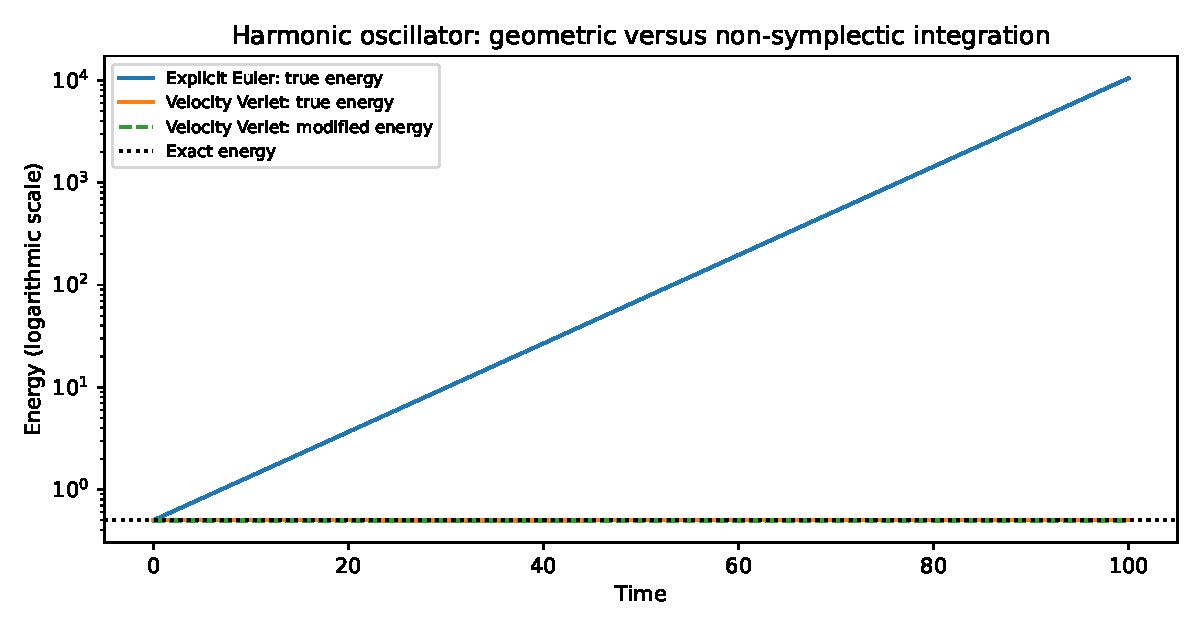
\includegraphics[width=.83\linewidth]{figures/hamiltonian_energy.pdf}
\caption{True and modified energies in the numerical Hamiltonian
benchmark. The $y$-axis is logarithmic; the modified Verlet energy is
constant up to roundoff, while Euler introduces an expanding phase-space
map and secular energy growth.}\label{fig:ham-energy}
\end{figure}
\begin{figure}[htbp]\centering
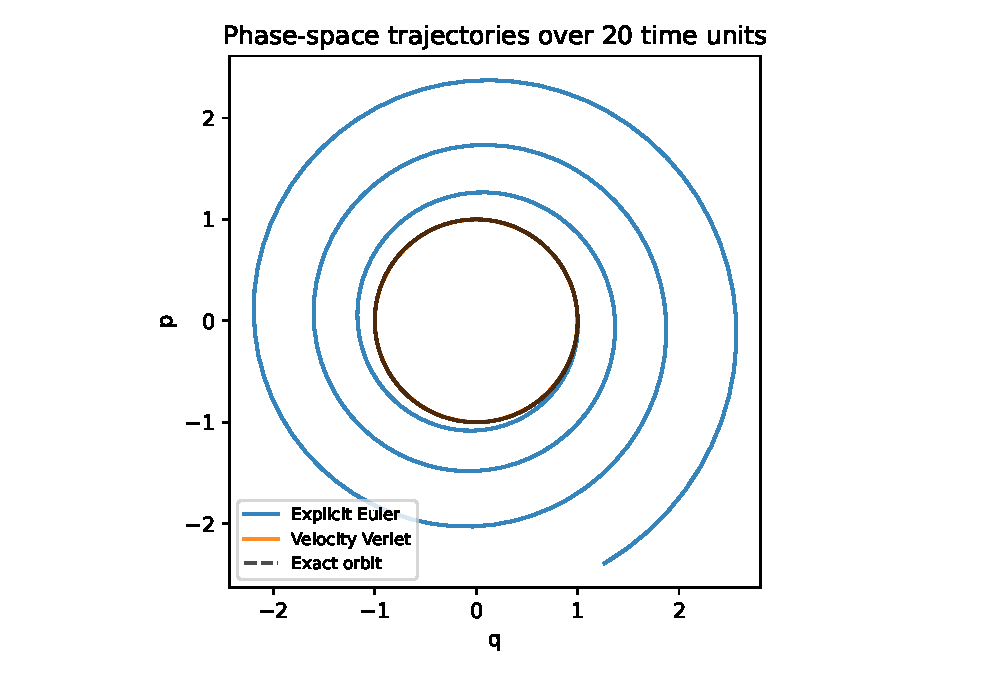
\includegraphics[width=.70\linewidth]{figures/hamiltonian_phase.pdf}
\caption{Exact, Euler, and Verlet trajectories in $(q,p)$ over
$0\le t\le20$. The differences arise from their discrete geometric
structures, not from the continuous Hamiltonian system.}
\label{fig:ham-phase}
\end{figure}


\paragraph{Entropy, Relative Entropy, and Free-Energy Principles}
\label{ch:entropy}
\paragraph{Differential entropy along a probability flow}
For a smooth strictly positive density define
$H(\rho)=-\int\rho\log\rho\dd x$.
We assume sufficient decay, integrability, and boundary conditions to
justify every integration by parts.

\begin{theorem}[Differential entropy balance under deterministic transport]
\label{thm:entropy}
\sourcecredit{9}{10}\phantomsection\label{src:p9q10}
If $\rho_t$ solves \eqref{eq:continuity} classically, then
\begin{equation}\label{eq:entropybalance}
 \frac{\dd}{\dd t}H(\rho_t)
 =\int\rho_t\nabla\!\cdot v_t\dd x
 =-\int\rho_t v_t\cdot\nabla\log\rho_t\dd x.
\end{equation}
\end{theorem}
\begin{proof}
Differentiate $-\int\rho_t\log\rho_t$ and insert
$\partial_t\rho_t=-\nabla\cdot(\rho_tv_t)$.
Mass conservation removes the integral of $\partial_t\rho_t$.
After integration by parts, the first identity follows; integrating
$\nabla\cdot(\rho_tv_t)$ once more yields the second.
\end{proof}

\begin{proposition}[Lagrangian score dynamics]
\label{prop:score}
\sourcecredit{9}{11}\phantomsection\label{src:p9q11}
Assume $v$ and $\log\rho$ are sufficiently smooth. Set
$s_t=\nabla\log\rho_t$. Along $\dot X_t=v_t(X_t)$,
\begin{equation}\label{eq:scoreflow}
 \frac{\dd}{\dd t}s_t(X_t)
 =-Dv_t(X_t)^\top s_t(X_t)
  -\nabla(\nabla\cdot v_t)(X_t).
\end{equation}
\end{proposition}
\begin{proof}
Divide \eqref{eq:continuity} by $\rho_t$ to obtain
$(\partial_t+v_t\cdot\nabla)\log\rho_t=-\nabla\cdot v_t$.
Taking a spatial gradient introduces the commutator
$\nabla(v_t\cdot\nabla f)
=Dv_t^\top\nabla f+(v_t\cdot\nabla)\nabla f$,
which gives \eqref{eq:scoreflow} along trajectories.
\end{proof}

\begin{corollary}[Transport of the log-density Hessian]
\label{ex:scorehessian}
Suppose $v\in C^3$ and $\ell_t=\log\rho_t$ is sufficiently smooth.
Writing $S_t=\nabla^2\ell_t$, $s_t=\nabla\ell_t$, and $A_t=Dv_t$,
the Hessian along a trajectory satisfies
\begin{equation}\label{eq:hessian-transport}
\begin{aligned}
\frac{\dd}{\dd t}S_t(X_t)
={}&-A_t(X_t)^\top S_t(X_t)-S_t(X_t)A_t(X_t)\\
&-\sum_{k=1}^d(s_t)_k(X_t)\nabla^2(v_t)_k(X_t)
-\nabla^2(\nabla\cdot v_t)(X_t).
\end{aligned}
\end{equation}
\end{corollary}
\begin{proof}
Take one more spatial derivative of
$(\partial_t+v\cdot\nabla)s=-Dv^\top s-\nabla(\nabla\cdot v)$.
For each index, differentiation of the material derivative contributes
$\partial_jv_k\,\partial_ks_i$. Differentiating the right side
contributes $-\partial_{ji}v_k\,s_k-\partial_iv_k\,\partial_js_k
-\partial_{ji}(\nabla\cdot v)$, giving \eqref{eq:hessian-transport}.
\end{proof}
\noindent For a global-in-time statement one additionally needs control of
the vector field and its derivatives, together with an appropriate
asymptotic stability or integrability argument. In the linear Gaussian
example below, these quantities can be computed from the covariance matrix.


\begin{example}[Long-time score need not converge]
For the one-dimensional contractive flow $\dot x_t=-\lambda x_t$
with $\lambda>0$ and $X_0\sim\mathcal N(0,\sigma_0^2)$,
$X_t=e^{-\lambda t}X_0$ and
$\rho_t=\mathcal N(0,\sigma_0^2e^{-2\lambda t})$. Therefore
\begin{equation}\label{eq:score-longtime}
 s_t(X_t)=-\frac{X_t}{\sigma_0^2e^{-2\lambda t}}
 =-\frac{e^{\lambda t}X_0}{\sigma_0^2},\qquad
 H(\rho_t)=H(\rho_0)-\lambda t.
\end{equation}
For any $X_0\neq0$ the Lagrangian score grows exponentially in magnitude,
even though the deterministic trajectories converge to the stable fixed
point. Global stability of the state dynamics is therefore not a
bounded-score theorem.
\end{example}

\paragraph{Relative entropy as an information functional}
For probability measures $\mu\ll\nu$ define
\begin{equation}\label{eq:kl}
 \KL(\mu\Vert\nu)=\int\log\left(\frac{\dd\mu}{\dd\nu}\right)\dd\mu,
\end{equation}
and set it to $+\infty$ when $\mu\not\ll\nu$.

\begin{theorem}[Gibbs' inequality]
\label{thm:kl}
\sourcecredit{11}{1}\phantomsection\label{src:p11q1}
For probability measures $\mu,\nu$, $\KL(\mu\Vert\nu)\geq0$, with equality
if and only if $\mu=\nu$.
\end{theorem}
\begin{proof}
If absolute continuity fails, the claim is immediate. Otherwise write
$r=\dd\mu/\dd\nu$. The inequality $r\log r-r+1\geq0$ for $r\geq0$
implies
$\KL(\mu\Vert\nu)=\int(r\log r-r+1)\dd\nu\geq0$.
Strict convexity, together with $\int r\dd\nu=1$, gives the equality case.
\end{proof}

\begin{theorem}[Gibbs variational identity]
\label{thm:gibbsvar}
\sourcecredit{11}{5}\phantomsection\label{src:p11q5}
Let $U$ be a bounded measurable function on a probability space
$(E,\nu)$. Set $Z_U=\int e^{-U}\dd\nu$ and $\nu_U=Z_U^{-1}e^{-U}\nu$.
For $\mu\ll\nu$ satisfying the relevant integrability conditions,
\begin{equation}\label{eq:gibbsvar}
 \KL(\mu\Vert\nu)+\int U\dd\mu
 =\KL(\mu\Vert\nu_U)-\log Z_U.
\end{equation}
Consequently, the infimum equals $-\log Z_U$ and is attained
at $\mu=\nu_U$.
\end{theorem}
\begin{proof}
Since $\log(\dd\nu_U/\dd\nu)=-U-\log Z_U$, the chain rule for
Radon--Nikodym derivatives gives
$\log(\dd\mu/\dd\nu_U)=
 \log(\dd\mu/\dd\nu)+U+\log Z_U$.
Integrate against $\mu$ and use Theorem~\ref{thm:kl}.
\end{proof}


\begin{theorem}[Donsker--Varadhan representation of relative entropy]
\label{thm:dv}
\sourcecredit{11}{6}\phantomsection\label{src:p11q6}
Let $\mu,\nu$ be probability measures on a measurable space. Then
\begin{equation}\label{eq:dv-variational}
\KL(\mu\Vert\nu)
=\sup_{g\in\mathcal B_b(E)}
\left\{\int_Eg\dd\mu-
\log\int_Ee^g\dd\nu\right\}.
\end{equation}
If $\mu\ll\nu$ and $g_*(x)=\log(\dd\mu/\dd\nu)(x)$ is a
permissible finite integrable test function, equality is attained
at $g_*+c$ for every constant $c$. In general the supremum over
bounded tests need not be attained.
\end{theorem}
\begin{proof}
For any bounded $g$, define the tilted probability
$\nu_g=e^g\nu/\int e^g\dd\nu$. The identity
\[
\KL(\mu\Vert\nu_g)
=\KL(\mu\Vert\nu)-\int g\dd\mu+
\log\int e^g\dd\nu
\]
whenever $\mu\ll\nu$ implies that the expression inside the supremum
is at most $\KL(\mu\Vert\nu)$. If $\mu\ll\nu$ and the entropy is
finite, choose
$g_n=\max(-n,\min(n,\log(\dd\mu/\dd\nu)))$.
For $r=\dd\mu/\dd\nu$, the functions $e^{g_n}$ converge to $r$
and satisfy $e^{g_n}\le r+1$, so $\int e^{g_n}\dd\nu\to1$ by
dominated convergence. Moreover $\int g_n\dd\mu\to\int\log r\dd\mu$
by truncation and integrability of $r\log r$.
The lower bound approaches $\KL(\mu\Vert\nu)$.
For infinite relative entropy, suitable bounded truncations similarly
make the right-hand side arbitrarily large. If $\mu\not\ll\nu$,
choose a set $A$ with $\mu(A)>0=\nu(A)$ and set $g=n\mathbf1_A$;
the variational expression grows like $n\mu(A)$.
This establishes equality also in the extended-real case.
\end{proof}

\begin{proposition}[Stein's integration-by-parts identity]
\label{prop:stein}
\sourcecredit{11}{8}\phantomsection\label{src:p11q8}
Let $\rho$ be positive and $C^1$ and let
$s=\nabla\log\rho$. If a scalar test function $f$ and $\rho$ decay
so that boundary terms vanish, then
\begin{equation}\label{eq:stein}
\mathbb E_\rho[\nabla f(X)+f(X)s(X)]=0.
\end{equation}
For $X\sim\mathcal N(0,I_d)$ this reads
$\mathbb E[Xf(X)]=\mathbb E[\nabla f(X)]$.
\end{proposition}
\begin{proof}
For each coordinate $i$,
$\int\partial_if\,\rho\dd x=-\int f\,\partial_i\rho\dd x
=-\int f\rho\,\partial_i\log\rho\dd x$.
For the standard Gaussian $\partial_i\log\rho=-x_i$.
The identity is exact, not an approximation that depends on
sampling or a neural network.
\end{proof}


\begin{theorem}[KL disintegration and data processing]
\label{thm:klchain}
\sourcecredit{11}{7}\phantomsection\label{src:p11q7}
Let $E,F$ be standard Borel spaces and consider disintegrations
\begin{align*}
 \mu(\dd x,\dd y)&=\mu_X(\dd x)\mu(\dd y\mid x),\\
 \nu(\dd x,\dd y)&=\nu_X(\dd x)\nu(\dd y\mid x).
\end{align*}
Under $\mu\ll\nu$,
\begin{align}\label{eq:klchain}
 \KL(\mu\Vert\nu)
 =\KL(\mu_X\Vert\nu_X)
 +\int_E\KL\big(\mu(\cdot\mid x)\Vert\nu(\cdot\mid x)\big)
 \mu_X(\dd x).
\end{align}
In particular, projection cannot increase KL divergence.
\end{theorem}
\begin{proof}
The density ratio factors almost everywhere into the marginal density
ratio and the conditional density ratio. Take its logarithm, integrate
with respect to $\mu$, and apply Fubini. Nonnegativity of the conditional
term yields the stated contraction.
\end{proof}

\begin{proposition}[Relative entropy of two transported densities]
\label{prop:kltransport}
\sourcecredit{9}{12}\phantomsection\label{src:p9q12}
Let positive smooth $\rho_t,\eta_t$ solve continuity equations with
velocities $v_t,w_t$, respectively, and suppose all boundary terms vanish.
Set $s_\rho=\nabla\log\rho_t$ and $s_\eta=\nabla\log\eta_t$. Then
\begin{equation}\label{eq:klflow}
 \frac{\dd}{\dd t}\KL(\rho_t\Vert\eta_t)
 =\int\rho_t(v_t-w_t)\cdot(s_\rho-s_\eta)\dd x.
\end{equation}
\end{proposition}
\begin{proof}
Differentiate $\int\rho\log(\rho/\eta)$, use mass conservation,
and insert both continuity equations. The $\rho$ contribution is
$\int\rho v\cdot(s_\rho-s_\eta)$. The $\eta$ contribution is
$\int\rho(\nabla\cdot w+w\cdot s_\eta)$,
which becomes $-\int\rho w\cdot(s_\rho-s_\eta)$ by integration by parts.
\end{proof}

\begin{Notice}[Sign check: Source Project 9 -- 12]
With the convention $\partial_t\rho=-\nabla\cdot(\rho v)$, the right side
of \eqref{eq:klflow} has a \emph{positive} prefactor. If another sign is
printed, it should be checked by differentiating the KL functional
rather than copied into the solution.
\end{Notice}

\paragraph{Thermodynamic free energy of a diffusion}
Consider the reversible overdamped Langevin equation
\begin{equation}\label{eq:langevin}
 \dd X_t=-\nabla V(X_t)\dd t+\sqrt{2\beta^{-1}}\dd W_t,
\end{equation}
with generator $\mathcal Lf=-\nabla V\cdot\nabla f+\beta^{-1}\Delta f$.
Under appropriate confining and no-flux/decay hypotheses,
$\pi(x)=Z^{-1}e^{-\beta V(x)}$ is an invariant density. Its forward equation is
\begin{equation}\label{eq:fp}
 \partial_t\rho_t=\nabla\cdot(\rho_t\nabla V)+\beta^{-1}\Delta\rho_t.
\end{equation}
Define the free-energy functional
$\mathcal F(\rho)=\int V\rho+\beta^{-1}\int\rho\log\rho$.
Direct substitution gives
\begin{equation}\label{eq:freekllink}
 \mathcal F(\rho)-\mathcal F(\pi)
 =\beta^{-1}\KL(\rho\Vert\pi),
\end{equation}
whenever the quantities are finite. For smooth solutions,
\begin{equation}\label{eq:freeenergy}
 \frac{\dd}{\dd t}\mathcal F(\rho_t)
 =-\int\rho_t\left|\nabla V+\beta^{-1}\nabla\log\rho_t\right|^2\dd x
 \leq0.
\end{equation}
To prove this, rewrite \eqref{eq:fp} as
$\partial_t\rho=\nabla\cdot\{\rho\nabla[\delta\mathcal F/\delta\rho]\}$,
with first variation $V+\beta^{-1}(\log\rho+1)$, then integrate by parts.
This is a smooth free-energy dissipation identity, not by itself an
existence theorem for infinite-dimensional metric gradient flows \cite{jko1998,villani2009}.

\section{Conditional Probability and Effective Dynamics}
\label{ch:coarsegraining}
\paragraph{Disintegration of a microscopic equilibrium measure}
Let $n\geq m\geq1$, and let $\xi:\R^n\to\R^m$ be $C^2$ with
$\operatorname{rank}D\xi(x)=m$ everywhere in the region of interest.
A \emph{reaction coordinate} is such a map selected to retain physically
relevant aspects of a higher-dimensional configuration. For a probability
measure $\mu$, write $\nu=\xi_\#\mu$. The disintegration theorem on
standard Borel spaces gives a family of probability kernels $\mu_z$,
defined for $\nu$-almost every $z$, such that
\begin{equation}\label{eq:disintegration}
 \int_{\R^n}f(x)g(\xi(x))\mu(\dd x)
 =\int_{\R^m}g(z)\left[\int_{\R^n}f(x)\mu_z(\dd x)\right]\nu(\dd z).
\end{equation}
The measure $\mu_z$ is supported on the level set
$\Sigma_z=\{x:\xi(x)=z\}$ for almost every $z$. The conditioning symbol
$\mu(\dd x\mid\xi(x)=z)$ represents this measure kernel, not an ordinary
Lebesgue density on $\R^n$.

\begin{example}[Gaussian conditional law for a coordinate average]
\label{ex:gaussianconditional}
\sourcecredit{12}{1}\phantomsection\label{src:p12q1}
Let $X\sim\mathcal N(0,I_n)$ and
$\xi(X)=n^{-1}\sum_{j=1}^nX_j=:Z$. Then
\begin{equation}\label{eq:gaussianconditional}
 Z\sim\mathcal N(0,n^{-1}),\qquad
 \Law(X\mid Z=z)=\mathcal N_{\Sigma_z}
 \left(z\mathbf 1, I_n-\tfrac1n\mathbf 1\mathbf 1^\top\right).
\end{equation}
The second Gaussian is \emph{degenerate} and supported on
$\{x:\mathbf 1^\top x=nz\}$.
\end{example}
\begin{proof}
Decompose $X$ into its orthogonal projections on
$\operatorname{span}\{\mathbf1\}$ and its orthogonal complement:
$X=Z\mathbf1+(I-n^{-1}\mathbf1\mathbf1^\top)X$. The two components are
independent jointly Gaussian vectors. Their means and covariances yield
\eqref{eq:gaussianconditional}.
\end{proof}


\paragraph{Noisy conditioning and the delta approximation.}
\sourcecredit{12}{2}\phantomsection\label{src:p12q2}
The geometry of conditioning on a sharp level set can be obtained as
a limit of ordinary, everywhere-defined Gaussian posteriors.
Let $X\sim\mathcal N(0,I_n)$, define
$Z=n^{-1}\mathbf1^\top X$, and observe $Y_\sigma=Z+\varepsilon$
with independent $\varepsilon\sim\mathcal N(0,\sigma^2)$.
The joint vector $(X,Y_\sigma)$ is Gaussian, with
$\operatorname{Cov}(X,Y_\sigma)=n^{-1}\mathbf1$ and
$\operatorname{Var}(Y_\sigma)=n^{-1}+\sigma^2$.
The Gaussian conditioning formula therefore yields
\begin{equation}\label{eq:noisy-gaussian-conditioning}
\begin{split}
\mathbb E[X\mid Y_\sigma=z]
&=\frac{z}{1+n\sigma^2}\mathbf1,\\
\operatorname{Cov}(X\mid Y_\sigma=z)
&=I_n-\frac{\mathbf1\mathbf1^\top}{n(1+n\sigma^2)}.
\end{split}
\end{equation}
As $\sigma\downarrow0$, the conditional mean and covariance converge
to the singular Gaussian law in Example~\ref{ex:gaussianconditional}.

For a general smooth reaction coordinate $\xi$ and an initial density
$\rho(x)$, Bayes' formula for the noisy observation
$Y_\sigma=\xi(X)+\sigma\zeta$ with independent standard Gaussian
$\zeta\in\R^m$ gives the posterior
\begin{equation}\label{eq:noisyposterior}
\mu_\sigma(\dd x\mid z)
=\frac{\rho(x)\varphi_{\sigma,m}(z-\xi(x))\dd x}
{\int\rho(y)\varphi_{\sigma,m}(z-\xi(y))\dd y},\qquad
\varphi_{\sigma,m}(u)=\frac{e^{-|u|^2/(2\sigma^2)}}{(2\pi\sigma^2)^{m/2}}.
\end{equation}
The kernels $\varphi_{\sigma,m}$ approximate the Dirac delta in the
\emph{reaction-coordinate variable}; for smooth nondegenerate $\xi$
and at regular values $z$, the posterior converges weakly under
suitable local integrability conditions to the disintegrated measure
on $\xi^{-1}(z)$. This is the precise meaning of the formal notation
$\delta(\xi(x)-z)\dd x$ and explains why the coarea Jacobian, rather
than ambient Lebesgue measure on the level set, appears in the limit.


\paragraph{Coarea representation of the marginal density}
For $x\in\R^n$ define the positive-definite Gram matrix
$G(x)=D\xi(x)D\xi(x)^\top\in\R^{m\times m}$ and
$J_\xi(x)=\sqrt{\det G(x)}$. Write
$\mathcal H^{n-m}\!\restriction_{\Sigma_z}$ for the $(n-m)$-dimensional
Hausdorff surface measure on $\Sigma_z$.

\begin{theorem}[Coarea disintegration and potential of mean force]
\label{thm:coarea}
\sourcecredit{12}{3}\phantomsection\label{src:p12q3}
Suppose $\mu(\dd x)=Z^{-1}e^{-\beta U(x)}\dd x$, where $\beta>0$,
$Z<\infty$, and the full-rank condition holds. Then $\nu=\xi_\#\mu$
has (almost-everywhere defined) density
\begin{equation}\label{eq:rhochannel}
 p_\xi(z)=\frac1Z\int_{\Sigma_z}
 \frac{e^{-\beta U(x)}}{J_\xi(x)}\dd\mathcal H^{n-m}(x),
\end{equation}
and the conditional kernel is the normalized surface measure
\begin{equation}\label{eq:conditionalsurface}
 \mu_z(\dd x)=\frac{e^{-\beta U(x)}J_\xi(x)^{-1}}{Zp_\xi(z)}
 \dd\mathcal H^{n-m}(x),\qquad x\in\Sigma_z.
\end{equation}
If $p_\xi(z)>0$, the free energy of the coordinate is
\begin{equation}\label{eq:potentialmeanforce}
 F(z)=-\beta^{-1}\log p_\xi(z).
\end{equation}
\end{theorem}
\begin{proof}
The coarea formula applied to the integrable function
$e^{-\beta U(x)}f(x)g(\xi(x))/Z$ gives
\begin{align*}
 &\int_{\R^n}f(x)g(\xi(x))\mu(\dd x)\\
 &\quad=\int_{\R^m}g(z)\left[\frac1Z\int_{\Sigma_z}
 \frac{f(x)e^{-\beta U(x)}}{J_\xi(x)}\dd\mathcal H^{n-m}(x)\right]\dd z.
\end{align*}
Set $f=1$ to identify the marginal density, then compare the expression
with \eqref{eq:disintegration} to identify the conditional kernel.
Equation~\eqref{eq:potentialmeanforce} is a definition; its additive
constant depends on the density convention and normalization.
\end{proof}

\begin{Notice}[Physical meaning of free energy]
The potential $F$ is associated with a \emph{probability measure on the
chosen coordinate space}. It is not simply the microscopic potential
$U$ evaluated on a representative configuration. Entropic contributions
arise from the number and geometry of microscopic states compatible with
$\xi(x)=z$. Changing coordinates changes the reference volume element,
and hence changes the density-based free-energy function.
\end{Notice}

\paragraph{The mean force from conditional expectation}
Let $G^{-1}$ denote the inverse Gram matrix and define vector fields
\begin{equation}\label{eq:Bi}
 B_i(x)=\sum_{j=1}^m[G(x)^{-1}]_{ij}\nabla\xi_j(x),
 \qquad D\xi(x)B_i(x)=e_i.
\end{equation}

\begin{theorem}[Mean-force identity]
\label{thm:meanforce}
\sourcecredit{12}{4}\phantomsection\label{src:p12q4}
Assume that $U,\xi$ are sufficiently smooth, the density $p_\xi$ is
positive and differentiable, and the following integrations by parts
have no boundary terms. Then for almost every $z$,
\begin{equation}\label{eq:meanforce}
 \partial_{z_i}F(z)
 =\E_\mu\left[B_i\cdot\nabla U-\beta^{-1}\nabla\cdot B_i
 \ \middle|\ \xi(X)=z\right].
\end{equation}
\end{theorem}
\begin{proof}
For a compactly supported smooth $\varphi$ on $\R^m$,
$B_i\cdot\nabla(\varphi\circ\xi)=\partial_{z_i}\varphi(\xi)$.
Integrating against $Z^{-1}e^{-\beta U(x)}\dd x$ and using integration
by parts yields
\begin{align*}
 \int\partial_{z_i}\varphi(z)p_\xi(z)\dd z
 &=\int B_i\cdot\nabla(\varphi\circ\xi)\mu(\dd x)\\
 &=\int\varphi(\xi(x))
 [\beta B_i\cdot\nabla U-\nabla\cdot B_i]\mu(\dd x).
\end{align*}
On the other hand, this equals $-\int\varphi(z)\partial_{z_i}p_\xi(z)\dd z$.
Disintegration identifies $-\partial_{z_i}\log p_\xi$ as the conditional
expectation in brackets. Multiplication by $\beta^{-1}$ gives the result.
\end{proof}

\medskip\noindent\textbf{Exercises and conceptual tests}\par
\begin{exercise}[Conditional geometry and normalization]
For a non-injective coordinate $\xi$, explain why the conditional
probability $\mu_z$ is naturally supported on a manifold, and why
writing $\mu(\xi(x)=z)$ as a point probability is misleading for
continuous laws. Verify the factors $Z$ and $J_\xi$ in
\eqref{eq:conditionalsurface}.
\end{exercise}
\begin{solution}
When $D\xi$ has rank $m<n$, the regular level-set theorem identifies
$\Sigma_z=\xi^{-1}(z)$ locally as a smooth submanifold of dimension
$n-m$. The conditional law is supported on that manifold for
$\nu$-almost every $z$. If $\nu$ has a Lebesgue density then
$\mathbb P(\xi(X)=z)=0$ for each fixed $z$; therefore the conditional
law must be understood through disintegration rather than as a naive
ratio of probabilities of two zero-probability events.

For a test function $g$ of the reduced variable, coarea gives
\begin{align*}
\mathbb E[g(\xi(X))]
&=\frac1Z\int_{\R^n}g(\xi(x))e^{-\beta U(x)}\dd x\\
&=\frac1Z\int_{\R^m}g(z)
\int_{\Sigma_z}\frac{e^{-\beta U(x)}}{J_\xi(x)}
\dd\mathcal H^{n-m}(x)\dd z.
\end{align*}
Thus $p_\xi(z)=Z^{-1}\int_{\Sigma_z}e^{-\beta U}/J_\xi
\dd\mathcal H^{n-m}$. For $p_\xi(z)>0$, the candidate conditional law
\eqref{eq:conditionalsurface} has mass
\[
\int_{\Sigma_z}\mu_z(\dd x)=
\frac{1}{Zp_\xi(z)}\int_{\Sigma_z}
\frac{e^{-\beta U(x)}}{J_\xi(x)}\dd\mathcal H^{n-m}(x)=1.
\]
The factor $Z$ originates in normalization of the original Gibbs
measure, whereas $J_\xi^{-1}$ arises from the geometry of slicing
Lebesgue volume into level sets. These are independent operations.
\end{solution}

\begin{exercise}[Mean force is not generally microscopic force]
Choose a nonlinear reaction coordinate with nonconstant $G(x)$.
Use \eqref{eq:meanforce} to identify the geometrical correction
$-\beta^{-1}\nabla\cdot B_i$. Discuss which terms would be lost by
approximating $\partial_{z_i}F$ with a single microscopic force sample.
\end{exercise}
\begin{solution}
For $\xi(x,y)=x+y^2$, the Gram scalar is $G=1+4y^2$ and
$B=(1,2y)/(1+4y^2)$. Hence
\begin{equation*}
\nabla\cdot B=\frac{2(1-4y^2)}{(1+4y^2)^2},
\end{equation*}
which is generically nonzero. The mean force includes both the
conditional average of $B\cdot\nabla U$ and the entropic/geometrical
term $-\beta^{-1}\E[\nabla\cdot B\mid\xi=z]$.
A force at one representative microscopic point contains neither the
conditional average nor the correct surface-volume contribution.
\end{solution}

\paragraph{Effective Dynamics and the Limits of Markovian Closure}
The marginal-projection viewpoint is closely related to the mimicking theorem of Gy\"ongy \cite{gyongy1986}.
\label{ch:effective}
\paragraph{Projection as a conditional least-squares problem}
The conditional expectation $\E[Y\mid\mathcal G]$ is the orthogonal
projection of any $Y\in L^2(\Omega)$ onto the closed subspace
$L^2(\mathcal G)$. This interpretation is the basis for learning effective
coefficients by regression.

\begin{proposition}[Law of total covariance]
\label{prop:totalcov}
\sourcecredit{13}{1}\phantomsection\label{src:p13q1}
For a square-integrable random vector $X$ and $Z=\xi(X)$,
\begin{equation}\label{eq:totalcov}
 \operatorname{Cov}(X)=
 \operatorname{Cov}(\E[X\mid Z])
 +\E[\operatorname{Cov}(X\mid Z)].
\end{equation}
\end{proposition}
\begin{proof}
Write $X-\E[X]=[\E(X\mid Z)-\E X]+[X-\E(X\mid Z)]$.
The mixed terms vanish after conditioning on $Z$. Expand the outer
product and take expectations.
\end{proof}

\begin{remark}
Principal component analysis minimizes mean-square reconstruction
error among linear projections and linear decoders for a centered
Gaussian vector, under the usual rank and orthogonality constraints.
The coordinate of largest equilibrium variance need not be the best
\emph{dynamical} reaction coordinate, since rare transitions and slow
time scales need not align with maximal variance.
\end{remark}

\medskip\noindent\textbf{Exercises}\par
\begin{exercise}[Choosing a physically meaningful coordinate]
For a centered Gaussian equilibrium law, formulate the constrained
rank-one projection problem that leads to the leading eigenvector of
the covariance. Then consider
$V(x_1,x_2)=\frac14(x_1^2-1)^2+\frac12x_2^2$:
compare a variance-based criterion with the kinetic importance of $x_1$
for inter-well transitions. State what additional dynamical criterion
would be needed to call a coordinate ``optimal.''
\end{exercise}
\begin{solution}
For a centered $X$ with covariance $\Sigma$ and a unit vector $u$,
minimizing the mean-square rank-one reconstruction error is equivalent to
\begin{equation*}
\min_{\|u\|=1}\E\|X-uu^\top X\|^2
=\operatorname{tr}\Sigma-\max_{\|u\|=1}u^\top\Sigma u.
\end{equation*}
The Rayleigh quotient is maximized by a top eigenvector of $\Sigma$.
For the double well, transitions between the two metastable basins
necessarily involve the $x_1$ coordinate, whereas $x_2$ relaxes
harmonically. Thus variance maximization is a static reconstruction
criterion; a dynamically appropriate coordinate must additionally
resolve the slow transition mode, for example through a committor
or a transfer-operator timescale criterion.
\end{solution}

\paragraph{The exact projected semimartingale equation}
For $\xi:\R^d\to\R$ of class $C^2$, apply It\^o calculus to
$Z_t^0=\xi(X_t)$ where $X_t$ solves \eqref{eq:langevin}.

\begin{theorem}[It\^o formula for a collective variable]
\label{thm:itoxi}
\sourcecredit{13}{2}\phantomsection\label{src:p13q2}
Assume sufficient regularity and non-explosion. Then
\begin{align}\label{eq:itoxi}
 \dd Z_t^0&=A_\xi(X_t)\dd t
 +\sqrt{2\beta^{-1}}\nabla\xi(X_t)\cdot\dd W_t,\\
 A_\xi(x)&=-\nabla V(x)\cdot\nabla\xi(x)+\beta^{-1}\Delta\xi(x).
\end{align}
The instantaneous quadratic variation is
$\dd[Z^0]_t=2\beta^{-1}|\nabla\xi(X_t)|^2\dd t$.
\end{theorem}
\begin{proof}
Write the microscopic equation in coordinates:
$\dd X_t^i=-\partial_iV(X_t)\dd t+
\sqrt{2\beta^{-1}}\dd W_t^i$.
The multidimensional It\^o formula says
\[
\dd\xi(X_t)=\sum_i\partial_i\xi(X_t)\dd X_t^i
+\frac12\sum_{i,j}\partial_{ij}\xi(X_t)\dd[X^i,X^j]_t.
\]
Because the Brownian components are independent,
$\dd[X^i,X^j]_t=2\beta^{-1}\delta_{ij}\dd t$.
Substitution gives
\begin{align*}
\dd\xi(X_t)&=-\sum_i\partial_i\xi\,\partial_iV\,\dd t
+\sqrt{2\beta^{-1}}\sum_i\partial_i\xi\,\dd W_t^i
+\beta^{-1}\sum_i\partial_{ii}\xi\,\dd t\\
&=\bigl(-\nabla V\cdot\nabla\xi+\beta^{-1}\Delta\xi\bigr)(X_t)\dd t
+\sqrt{2\beta^{-1}}\nabla\xi(X_t)\cdot\dd W_t.
\end{align*}
The martingale part has quadratic variation
$2\beta^{-1}\int_0^t|\nabla\xi(X_s)|^2\dd s$, so its
instantaneous variance coefficient is the \emph{squared magnitude}
$|\nabla\xi|^2$. Averaging the amplitude $|\nabla\xi|$ instead
would not preserve this quadratic-variation identity.
\end{proof}

\paragraph{A Markov model with the same one-time marginals}
Write $\nu_t=\Law(Z_t^0)$ and define versions of conditional moments
\begin{align}\label{eq:projectedcoeffs}
 b(t,z)&=\E[A_\xi(X_t)\mid\xi(X_t)=z],\\
 a(t,z)&=\E[|\nabla\xi(X_t)|^2\mid\xi(X_t)=z].
\end{align}
The first moment and the quadratic variation both matter: averaging the
noise \emph{amplitude} is generally not equivalent to averaging its square.

\begin{theorem}[Projected time marginals]
\label{thm:mimic}
\sourcecredit{13}{3}\phantomsection\label{src:p13q3}
Suppose $b,a$ in \eqref{eq:projectedcoeffs} admit a non-explosive weak
solution of
\begin{equation}\label{eq:projectedsde}
 \dd Y_t=b(t,Y_t)\dd t+\sqrt{2\beta^{-1}a(t,Y_t)}\dd B_t,
 \qquad\Law(Y_0)=\Law(\xi(X_0)),
\end{equation}
and assume uniqueness in the class of measure-valued solutions to its
forward Fokker--Planck equation. Then, for all times covered by these
assumptions,
\begin{equation}\label{eq:marginalmatch}
 \Law(Y_t)=\Law(\xi(X_t)).
\end{equation}
This does not assert equality of path laws.
\end{theorem}
\begin{proof}
For each $\varphi\in C_c^\infty(\R)$, Theorem~\ref{thm:itoxi}
and conditional expectation show that
\begin{equation}\label{eq:projectedweak}
 \frac{\dd}{\dd t}\int\varphi(z)\nu_t(\dd z)
 =\int\big[b(t,z)\varphi'(z)+\beta^{-1}a(t,z)\varphi''(z)\big]\nu_t(\dd z).
\end{equation}
The law of \eqref{eq:projectedsde} satisfies exactly the same weak equation
and initial condition. By the stipulated uniqueness of the forward
problem their laws coincide at each $t$.
\end{proof}

\begin{Notice}[What this theorem does not prove]
The argument proves a conditional implication: \emph{if} a diffusion
with the projected coefficients exists and the forward equation is
unique in the relevant class, its one-time marginals match.
The weak calculation alone is not an existence theorem. Moreover,
$\xi(X_t)$ need not be Markov, and equality of $\nu_t$ for all $t$ does
not imply equality of $\E[Z_sZ_t]$, hitting-time statistics, or pathwise
entropy production.
\end{Notice}

\paragraph{Static closure, dynamic projection, and memory}
A common equilibrium approximation uses the conditional equilibrium law
$\mu_z=\mu(\dd x\mid\xi(x)=z)$ to define
$\bar b_{\mathrm{eq}}(z)=\int A_\xi(x)\mu_z(\dd x)$.
For a system away from equilibrium, however, the correct coefficients
$\bar b(t,z)$ in \eqref{eq:projectedcoeffs} depend on the evolving law
$\rho_t$, not solely on the equilibrium Gibbs measure. Replacing
conditional distributions at time $t$ by equilibrium conditionals is
therefore a modeling assumption, not an identity. A memory-kernel
formulation is another possible reduction route, but is beyond our
present minimal theorem package.

\section{Learned Flows and Structure-Preserving Approximation}
\label{ch:learnedflows}
\paragraph{The probability-current velocity}
Assume $\rho_t(x)>0$ is a sufficiently smooth density solving the
Fokker--Planck equation \eqref{eq:fp}. Define the probability current
$J_t(x)=-\rho_t(x)\nabla V(x)-\beta^{-1}\nabla\rho_t(x)$ and its current
velocity
\begin{equation}\label{eq:currentvelocity}
 v_t^{\mathrm{cur}}(x):=\frac{J_t(x)}{\rho_t(x)}
 =-\nabla V(x)-\beta^{-1}\nabla\log\rho_t(x).
\end{equation}
Then $\partial_t\rho_t+\nabla\cdot(\rho_tv_t^{\mathrm{cur}})=0$.
This identity links stochastic evolution to the deterministic continuity
equation in Chapter~\ref{ch:foundations}. If the velocity generates a
well-defined flow with suitable regularity, it can transport the same
\emph{one-time densities} as the diffusion. It does not reproduce
Brownian sample paths, quadratic variation, or their multi-time laws.

\paragraph{Stochastic interpolation and conditional velocity}
Let $(X_0,X_1)$ have a joint law $\gamma$ on $\R^d\times\R^d$, with
prescribed marginals $\rho_0,\rho_1$. Suppose $\alpha,\lambda$ are
$C^1$ functions on $[0,1]$ with
$\alpha_0=1,\alpha_1=0,\lambda_0=0,\lambda_1=1$, and set
\begin{equation}\label{eq:interpolant}
 I_t=\alpha_tX_0+\lambda_tX_1.
\end{equation}
The joint law $\gamma$ is a \emph{coupling}; its choice affects the
path $t\mapsto\Law(I_t)$ and the velocity required to transport it.


\begin{example}[Exact Gaussian interpolation: single and two-time laws]
\label{ex:gaussian-interpolants}
\sourcecredit{14}{1}\phantomsection\label{src:p14q1}
Assume $X_0$ and $X_1$ are independent standard Gaussian vectors in
$\R^d$. Then
$I_t=\alpha_tX_0+\lambda_tX_1$ is centered Gaussian, and independence
makes the covariance calculation explicit:
\begin{align}\label{eq:gaussian-interpolant-statistics}
\operatorname{Cov}(I_t)&=(\alpha_t^2+\lambda_t^2)I_d,\\
\operatorname{Cov}(I_s,I_t)&=(\alpha_s\alpha_t+\lambda_s\lambda_t)I_d.\notag
\end{align}
Indeed, expand $\mathbb E[I_sI_t^\top]$ into four terms.
The cross terms vanish because the endpoint Gaussians are independent
and centered, while $\mathbb E[X_iX_i^\top]=I_d$.
For the linear interpolation $\alpha_t=1-t$, $\lambda_t=t$,
we find $I_t\sim\mathcal N(0,[(1-t)^2+t^2]I_d)$, which is narrower
at $t=1/2$ than at either endpoint. Thus even an interpolation between
identical endpoint marginals need not have constant intermediate
marginals, and the coupling is mathematically consequential.
\end{example}


\begin{theorem}[Conditional interpolation velocity]
\label{thm:interpolant}
\sourcecredit{14}{2}\phantomsection\label{src:p14q2}
Assume $\E(|X_0|+|X_1|)<\infty$ and that the following distributional
derivatives are legitimate. Let $\rho_t=\Law(I_t)$ and define a version of
\begin{equation}\label{eq:interpolantvelocity}
 v_t(z)=\E[\dot\alpha_tX_0+\dot\lambda_tX_1\mid I_t=z].
\end{equation}
Then the continuity equation
$\partial_t\rho_t+\nabla\cdot(\rho_tv_t)=0$ holds weakly.
\end{theorem}
\begin{proof}
For $\varphi\in C_c^1(\R^d)$,
$\frac{\dd}{\dd t}\E\varphi(I_t)
=\E[\nabla\varphi(I_t)\cdot\dot I_t]$.
Conditioning on $I_t$ gives
$\int\nabla\varphi(z)\cdot v_t(z)\rho_t(\dd z)$, the desired weak
continuity equation.
\end{proof}

\begin{remark}[Nonuniqueness of transporting velocity]
On a domain with suitable boundary conditions, if $v_t$ transports
$\rho_t$, so does $v_t+w_t$ whenever
$\nabla\cdot(\rho_tw_t)=0$ in distributions.
Thus a density path alone does not uniquely determine an ambient
velocity field. The conditional construction in
\eqref{eq:interpolantvelocity} supplies a \emph{particular} velocity;
its uniqueness requires further criteria such as an appropriate
minimal-action principle or a one-dimensional zero-flux condition.
\end{remark}


\begin{proposition}[Conditional score identity for Gaussian interpolation]
\label{prop:interpolant-score}
\sourcecredit{14}{3}\phantomsection\label{src:p14q3}
Suppose $X_0\sim\mathcal N(0,I_d)$ is independent of an arbitrary
random vector $X_1$, and $I_t=\alpha_tX_0+\lambda_tX_1$ with
$\alpha_t\ne0$. Then $I_t$ has a smooth strictly positive density
$\rho_t$ and
\begin{equation}\label{eq:conditional-score}
\nabla\log\rho_t(x)
=-\frac1{\alpha_t}\mathbb E[X_0\mid I_t=x].
\end{equation}
If both endpoints are independent standard Gaussians, the right side
reduces to $-x/(\alpha_t^2+\lambda_t^2)$.
\end{proposition}
\begin{proof}
Conditioning on $X_1=y$ shows that $I_t$ has Gaussian density
$\varphi_{|\alpha_t|}(x-\lambda_ty)$. Hence
\[
\rho_t(x)=\int\varphi_{|\alpha_t|}(x-\lambda_ty)\mu_1(\dd y).
\]
Gaussian convolution permits differentiation under the integral:
\[
\nabla\rho_t(x)=-\frac1{\alpha_t^2}
\int(x-\lambda_ty)\varphi_{|\alpha_t|}(x-\lambda_ty)
\mu_1(\dd y).
\]
Divide by $\rho_t(x)$ and recognize the conditional expectation
$\mathbb E[x-\lambda_tX_1\mid I_t=x]=
\alpha_t\mathbb E[X_0\mid I_t=x]$.
The formula is therefore a Gaussian integration identity, not a
general claim for arbitrary endpoint coupling. For standard independent
Gaussian endpoints, elementary joint-Gaussian conditioning gives
$\mathbb E[X_0\mid I_t=x]=\alpha_tx/(
\alpha_t^2+\lambda_t^2)$.
\end{proof}


\paragraph{Conditional regression as an AI component}
For a square-integrable observable $G_t=G(X_t)$, the variational identity
\begin{equation}\label{eq:regression}
 g_t^*=\arg\min_{g\in L^2(\Law(Z_t))}
 \E|g(Z_t)-G_t|^2
 =\E[G_t\mid Z_t=\cdot]
\end{equation}
is understood as equality of equivalence classes almost everywhere.
This conditional regression is also the population objective used in flow matching and stochastic-interpolant methods \cite{lipman2023,albergo2025}. A neural network can parameterize $g_\theta(t,z)$ to approximate an
effective drift or conditional velocity. The learning problem is not
mathematically identical to the population optimum: finite samples,
representation restrictions, and optimization errors introduce additional
approximation layers.

\medskip\noindent\textbf{Exercises and research tasks}\par


\begin{exercise}[Same marginal flow, different path statistics]
Construct a stationary one-dimensional diffusion and a deterministic
current-velocity flow with identical one-time densities. Compare their
quadratic variations and two-time correlations. Explain why no
comparison based exclusively on $\rho_t$ can detect the discrepancy.
\end{exercise}
\begin{solution}
Fix $\gamma>0$. Consider the stationary Ornstein--Uhlenbeck diffusion
\[
\dd X_t=-\gamma X_t\dd t+\sqrt{2\gamma}\dd W_t,
\qquad X_0\sim\mathcal N(0,1),
\]
with the initial state independent of the driving Brownian motion.
Its invariant density is the standard Gaussian $\rho(x)$, so
$\rho_t=\rho$ at every $t$. Its probability current is
$J=-\gamma x\rho-\gamma\rho'$. Since $\rho'=-x\rho$, this
current vanishes, and the associated deterministic current velocity
$v=J/\rho$ is identically zero.

Let $Y_0\sim\mathcal N(0,1)$ and define the deterministic flow
$Y_t=\Phi_t(Y_0)=Y_0$, where $\Phi_t(x)=x$ solves $\dot y=0$.
Both processes therefore have the same law $\mathcal N(0,1)$ at
each fixed time. Their path statistics differ sharply:
\begin{align*}
[X]_t&=2\gamma t, & [Y]_t&=0,\\
\mathbb E[X_sX_t]&=e^{-\gamma|t-s|}, &
\mathbb E[Y_sY_t]&=1.
\end{align*}
The OU covariance follows by solving the linear SDE for $t\ge s$:
\[
X_t=e^{-\gamma(t-s)}X_s+
\sqrt{2\gamma}\int_s^te^{-\gamma(t-r)}\dd W_r.
\]
The stochastic integral is independent of $X_s$ with mean zero, hence
\[
\mathbb E[X_sX_t]=e^{-\gamma(t-s)}\mathbb E[X_s^2].
\]
In contrast the deterministic process is constant along each path.
Thus matching all one-time densities cannot establish either equal
quadratic variation or equal two-time correlations.
\end{solution}


\paragraph{Variational transport, target laws, and learned flow construction.}
A learned probability flow can be chosen by minimizing a mismatch
between an initial law transported by a map and a prescribed target
law. The dependence of a density on the transporting map is nonlinear;
therefore a small perturbation of the map must be propagated through
its pushforward, rather than differentiated as if density and map were
independent.

\begin{theorem}[First variation of a pushforward KL objective]
\label{thm:flow-kl-variation}
\sourcecredit{9}{13}\phantomsection\label{src:p9q13}
Let $\rho_0$ and $q$ be smooth positive probability densities on
$\R^d$, and let $F$ be an orientation-preserving $C^2$
diffeomorphism with $\rho=F_\#\rho_0$. Put
$\mathcal J(F)=\KL(q\Vert\rho)$. For a compactly supported smooth
vector field $w$, perturb $F$ through
$F_\varepsilon=(\mathrm{id}+\varepsilon w)\circ F$.
If differentiation under the integral is justified, then
\begin{equation}\label{eq:flow-kl-first-variation}
\frac{\dd}{\dd\varepsilon}\mathcal J(F_\varepsilon)
\Big|_{\varepsilon=0}
=\int_{\R^d}q(y)
[\nabla\log\rho(y)-\nabla\log q(y)]\cdot w(y)\dd y.
\end{equation}
Equivalently, for a Lagrangian map perturbation
$\delta F(x)=w(F(x))$,
\begin{equation}\label{eq:flow-kl-lagrangian}
\delta\mathcal J
=\int_{\R^d}q(F(x))\det DF(x)
[\nabla\log\rho-\nabla\log q](F(x))
\cdot\delta F(x)\dd x.
\end{equation}
\end{theorem}
\begin{proof}
For any compactly supported test function $\varphi$,
\begin{align*}
\int\varphi(y)\rho_\varepsilon(y)\dd y
&=\int\varphi(y+\varepsilon w(y))\rho(y)\dd y,\\
\left.\frac{\dd}{\dd\varepsilon}\right|_0
\int\varphi\rho_\varepsilon\dd y
&=\int\nabla\varphi(y)\cdot w(y)\rho(y)\dd y
=-\int\varphi\nabla\cdot(\rho w)\dd y.
\end{align*}
Therefore $\delta\rho=-\nabla\cdot(\rho w)$ in the
sense of distributions. Since $q$ is fixed,
\[
\delta\mathcal J
=-\int q(y)\frac{\delta\rho(y)}{\rho(y)}\dd y
=\int q(y)\left[\nabla\cdot w(y)
+w(y)\cdot\nabla\log\rho(y)\right]\dd y.
\]
Integrate the divergence term by parts to obtain
$\int q\nabla\cdot w=-\int q\,w\cdot\nabla\log q$.
This proves \eqref{eq:flow-kl-first-variation}.
Finally, set $y=F(x)$ so that
$\dd y=\det DF(x)\dd x$ and
$w(y)=\delta F(F^{-1}(y))$, giving
\eqref{eq:flow-kl-lagrangian}. The factor $\det DF$ is necessary
when expressing the variation relative to the initial-coordinate
Lebesgue measure; omitting it mixes Eulerian and Lagrangian
representations.
\end{proof}

\begin{example}[Constructing a transport toward a tilted Gaussian law]
\label{ex:target-transport}
\sourcecredit{9}{14}\phantomsection\label{src:p9q14}
Let $\rho_0$ denote the standard Gaussian density in one dimension,
let $h\ge0$ be measurable, and assume
$0<Z_h=\int h(x)\rho_0(x)\dd x<\infty$.
The desired density is $\rho_h(x)=h(x)\rho_0(x)/Z_h$.
With cumulative distribution functions
\[
F_0(x)=\int_{-\infty}^x\rho_0(u)\dd u,
\qquad F_h(z)=\int_{-\infty}^z\rho_h(u)\dd u,
\]
the quantile transport
\begin{equation}\label{eq:quantile-transport}
T(x)=F_h^{-1}(F_0(x))
\end{equation}
satisfies $T_\#(\rho_0\dd x)=\rho_h\dd x$.
Indeed, $F_0(X_0)$ is uniform on $(0,1)$ for $X_0\sim\rho_0$,
and the generalized inverse $F_h^{-1}$ converts a uniform variable
into the distribution with CDF $F_h$.
If $T$ is sufficiently smooth and strictly increasing, the maps
$T_t(x)=(1-t)x+tT(x)$ are strictly increasing for $0\le t\le1$,
and their (possibly time-dependent) velocity is explicitly
\begin{equation}\label{eq:quantile-flow-velocity}
v_t(z)=(T-\mathrm{id})(T_t^{-1}(z)),\qquad
\partial_tT_t(x)=v_t(T_t(x)).
\end{equation}
Thus $T_0=\mathrm{id}$ and $T_1=T$ give a flow transporting the
initial law to the target. In multiple dimensions a triangular
Knothe--Rosenblatt rearrangement gives an explicit recursive
construction when the source and target have strictly positive
conditional densities. Denote by $F_{0,1}$ and $F_{h,1}$ the first
coordinate CDFs, and by $F_{0,i\mid 1:i-1}$ and
$F_{h,i\mid 1:i-1}$ the conditional CDFs of coordinate $i$ given
its predecessors. Set
\begin{align*}
T_1(x_1)&=F_{h,1}^{-1}(F_{0,1}(x_1)),\\
T_i(x_1,\ldots,x_i)&=
 F_{h,i\mid 1:i-1}^{-1}
 \left(F_{0,i\mid 1:i-1}(x_i\mid x_1,\ldots,x_{i-1})
 \mid T_1(x),\ldots,T_{i-1}(x)\right).
\end{align*}
The second line means the inverse target conditional CDF evaluated
at the already transported preceding coordinates. By induction,
these triangular conditional transformations transport the joint
source law to the target law \cite{villani2009}. A smooth global
flow whose time-one map equals this measurable rearrangement
requires additional regularity and invertibility; the existence of
a measurable transport by itself does not imply such a flow.
If $h$ vanishes on an open set, the target may have support gaps, and
a global smooth diffeomorphism of a strictly positive full-support
Gaussian cannot in general produce that density exactly.

If only samples of the initial or target law are available, neither
$F_0$ nor $F_h$ is known exactly. Empirical CDFs, conditional density
models, flow matching, or learned monotone maps provide approximations;
finite training samples do not identify a unique exact population
transport. Validations should use independent samples and report
both distributional discrepancies and dynamical quantities relevant
to the intended application.
\end{example}

\begin{proposition}[Formal optimality system for a kinetic-action flow]
\label{prop:kinetic-control}
\sourcecredit{9}{15}\phantomsection\label{src:p9q15}
Let $\rho_0$ be prescribed and let $\mathcal E(\rho_1)$ be a specified,
differentiable terminal functional of the final probability law.
Consider, formally under sufficient smoothness,
\begin{equation}\label{eq:benamou-terminal}
\min_{\rho,v}\left\{
\int_0^1\int_{\R^d}\tfrac12\rho_t(x)|v_t(x)|^2\dd x\dd t
+\mathcal E(\rho_1)\right\},\qquad
\partial_t\rho+\nabla\cdot(\rho v)=0.
\end{equation}
A smooth interior stationary point with positive density admits a
multiplier $\phi$ satisfying
\begin{equation}\label{eq:kinetic-optimality}
v_t=\nabla\phi_t,\qquad
\partial_t\phi_t+\tfrac12|\nabla\phi_t|^2=0,
\qquad
\phi_1=-\frac{\delta\mathcal E}{\delta\rho}(\rho_1),
\end{equation}
along with the continuity equation and the initial condition.
The original assessment leaves the terminal functional unspecified;
therefore it does not determine a unique optimal flow without an
additional choice of $\mathcal E$.
\end{proposition}
\begin{proof}
Enforce the continuity equation with a smooth multiplier $\phi$:
\[
\mathfrak L=\int_0^1\int\left[\tfrac12\rho|v|^2+
\phi\bigl(\partial_t\rho+\nabla\cdot(\rho v)\bigr)\right]\dd x\dd t
+\mathcal E(\rho_1).
\]
Integration by parts in time and space gives
\[
\mathfrak L=\int_0^1\int\rho
\left[\tfrac12|v|^2-\partial_t\phi-v\cdot\nabla\phi\right]
\dd x\dd t
+\int\phi_1\rho_1\dd x-\int\phi_0\rho_0\dd x
+\mathcal E(\rho_1).
\]
The first variation in $v$ is
$\int\rho(v-\nabla\phi)\cdot\delta v$, implying
$v=\nabla\phi$ when $\rho>0$.
The interior variation in $\rho$ gives
$\tfrac12|v|^2-\partial_t\phi-v\cdot\nabla\phi=0$;
substituting the velocity gives
$\partial_t\phi+\tfrac12|\nabla\phi|^2=0$.
Finally, variations of the terminal density produce
$\phi_1+\delta\mathcal E/\delta\rho=0$ (up to an additive
mass-constraint constant). These are necessary first-order conditions;
they do not by themselves prove existence, uniqueness, or global
optimality of a smooth solution.
\end{proof}

\begin{example}[Explicit solution for one particle with quadratic terminal cost]
To illustrate the terminal optimality condition, restrict to a
single deterministic path with $\gamma(0)=y$ and minimize
\[
\frac12\int_0^1|\dot\gamma(t)|^2\dd t
+\frac\kappa2|\gamma(1)-z_*|^2,\qquad\kappa>0.
\]
For fixed endpoint $z_1$, Cauchy--Schwarz gives the minimizing
straight line $\gamma(t)=y+t(z_1-y)$, whose cost is
$\frac12|z_1-y|^2+\frac\kappa2|z_1-z_*|^2$.
Differentiation with respect to $z_1$ gives
$(z_1-y)+\kappa(z_1-z_*)=0$, so
\[
z_1=\frac{y+\kappa z_*}{1+\kappa},\qquad
\gamma_*(t)=y+\frac{t\kappa}{1+\kappa}(z_*-y).
\]
This makes the role of the terminal functional explicit: the path
does not in general reach $z_*$ exactly, but balances kinetic cost
against the specified terminal penalty.
\end{example}


\paragraph{Structure-Preserving Numerical Probability Evolution}
The Markov generator structure is central to numerical approximations of Fokker--Planck dynamics \cite{pavliotis2014}.
\label{ch:numerical}
\paragraph{A finite-volume Markov-chain discretization}
Consider on the bounded interval $[0,1]$ the Fokker--Planck equation
\begin{equation}\label{eq:fpbounded}
 \partial_t p=\partial_x(V'p)+D\partial_{xx}p,\qquad D=\tfrac12,
\end{equation}
with \emph{zero-flux} boundary condition
$J=-V'p-Dp'=0$ at $x=0,1$. These conditions ensure total mass
conservation for a general nonconstant potential; plain $p'=0$ does
not imply $J=0$ when $V'$ is nonzero at a boundary.
Divide $[0,1]$ into cells $I_i$ of width $h=1/N$ with centers $x_i$.
Let $m_i(t)\approx\int_{I_i}p(t,x)\dd x$ denote \emph{cell masses}, not
pointwise densities. Set $V_i=V(x_i)$ and nearest-neighbor rates
\begin{equation}\label{eq:markovrates}
 k_{i,i+1}=\frac{D}{h^2}
 \exp\left[-\frac{V_{i+1}-V_i}{2D}\right],\qquad
 k_{i+1,i}=\frac{D}{h^2}
 \exp\left[\frac{V_{i+1}-V_i}{2D}\right].
\end{equation}
No transitions are permitted beyond the two boundary cells.

\begin{theorem}[Positivity, conservation, and detailed balance]
\label{thm:markovfv}
\sourcecredit{8}{Main task}\phantomsection\label{src:p8main}
Let the semidiscrete cell-mass vector satisfy
\begin{equation}\label{eq:markovfv}
 \dot m_i=\sum_{j\neq i}(k_{j,i}m_j-k_{i,j}m_i),
 \qquad m_i(0)\geq0,\quad\sum_i m_i(0)=1,
\end{equation}
with the rates in \eqref{eq:markovrates}. Then
$m_i(t)\geq0$ and $\sum_i m_i(t)=1$ for all $t\geq0$.
Moreover, $\pi_i=Z_h^{-1}e^{-V_i/D}$ is stationary and satisfies
detailed balance: $\pi_i k_{i,j}=\pi_jk_{j,i}$.
\end{theorem}
\begin{proof}
The matrix of \eqref{eq:markovfv} has nonnegative off-diagonal
entries and columns summing to zero, so its exponential is stochastic
and preserves nonnegative cell masses. Summing \eqref{eq:markovfv}
over $i$ cancels every internal flux. Finally,
$k_{i,i+1}/k_{i+1,i}
=\exp[-(V_{i+1}-V_i)/D]=\pi_{i+1}/\pi_i$.
\end{proof}

\begin{proposition}[Discrete relative-entropy dissipation]
Suppose $m_i(t)>0$ and write $r_i=m_i/\pi_i$. Then
\begin{equation}\label{eq:discreteent}
 \frac{\dd}{\dd t}\sum_i m_i\log\frac{m_i}{\pi_i}
 =-\sum_{i=1}^{N-1}\pi_i k_{i,i+1}
 (r_{i+1}-r_i)(\log r_{i+1}-\log r_i)\leq0.
\end{equation}
\end{proposition}
\begin{proof}
Differentiate the entropy, substitute \eqref{eq:markovfv},
and group each pair $i,i+1$. The detailed-balance identity makes its
coefficient symmetric, and the monotonicity of $\log$ gives the sign.
\end{proof}

\medskip\noindent\textbf{Exercise: examine the original scheme}\par
\begin{exercise}[The central-difference positivity test]
\label{ex:centralpositivity}
\sourcecredit{8}{1}\phantomsection\label{src:p8q1}
The assessment proposes a centered approximation for the drift--diffusion
PDE with ghost-cell boundary values. Rewrite it as an ODE for cell masses;
determine whether the off-diagonal entries are nonnegative and whether
the boundary closure conserves total mass.
\end{exercise}
\begin{solution}
Put $b_i=-V'(x_i)$, $p_i\approx p(t,x_i)$, and $m_i=hp_i$.
For an interior site, the centered stencil becomes
\begin{equation}\label{eq:centered-generator}
\dot m_i=
\left(\frac D{h^2}+\frac{b_{i-1}}{2h}\right)m_{i-1}
-\frac{2D}{h^2}m_i
+\left(\frac D{h^2}-\frac{b_{i+1}}{2h}\right)m_{i+1}.
\end{equation}
To have nonnegative off-diagonal entries on all interior interfaces,
a sufficient interior criterion is $|b_j|h/(2D)\le1$. This is the
cell P\'eclet condition. It alone does not make the matrix a Markov
generator, because its column sums must also vanish. Indeed, with the
proposed density ghost cells $p_0=p_1$ and $p_{N+1}=p_N$ and with the
natural extrapolation $b_0=b_1$, $b_{N+1}=b_N$, summation yields
\begin{equation}\label{eq:centered-mass}
\frac{\dd}{\dd t}\sum_{i=1}^Nm_i(t)
=-\frac{b_Nm_N-b_1m_1}{h},
\end{equation}
which is not zero in general. Without boundary values for $b_0$ and
$b_{N+1}$ the source stencil is not even fully specified at the end
cells. By contrast, the rates \eqref{eq:markovrates} define a genuine
nearest-neighbor Markov generator with nonnegative transitions and
zero column sums for arbitrary potential differences. Thus formal
centered consistency, stochastic positivity, and no-flux conservation
are three distinct questions.
\end{solution}

\paragraph{Verification protocol}
The numerical study should monitor (i) total mass and sign of each cell
mass, (ii) convergence of the semidiscrete solution under mesh refinement,
(iii) equilibrium detailed balance and entropy dissipation, and
(iv) discrepancy against an analytic solution or an independent finer-grid
reference. A low loss on finitely many collocation points, by itself, is not
a proof of a global density approximation.

\section{A Coupled OU Benchmark: Exact, Numerical, and AI Results}
\label{ch:benchmark}
\paragraph{The microscopic model and its Gibbs equilibrium}
For $a,c,\beta>0$ and $\kappa\in\R$, consider
\begin{equation}\label{eq:ouV}
 V(x,y)=\frac a2x^2+\frac c2(y-\kappa x)^2,
 \qquad\xi(x,y)=x.
\end{equation}
Writing $R_t=(X_t,Y_t)^\top$, the microscopic SDE becomes
\begin{equation}\label{eq:ouSDE}
 \dd R_t=-K R_t\dd t+\sqrt{2\beta^{-1}}\dd W_t,
 \quad K=\begin{pmatrix}a+c\kappa^2&-c\kappa\\-c\kappa&c\end{pmatrix}.
\end{equation}
Since $\det K=ac>0$, $K$ is symmetric positive definite.

\begin{proposition}[Gaussian equilibrium and projected free energy]
\label{prop:oueq}
The unique invariant law of \eqref{eq:ouSDE} is
$\mathcal N(0,\Sigma_\infty)$, where
\begin{equation}\label{eq:oucov}
 \Sigma_\infty=\beta^{-1}K^{-1}
 =\beta^{-1}\begin{pmatrix}
 1/a&\kappa/a\\[2pt]\kappa/a&1/c+\kappa^2/a
 \end{pmatrix}.
\end{equation}
At equilibrium,
$X\sim\mathcal N(0,(\beta a)^{-1})$ and
$Y\mid X=z\sim\mathcal N(\kappa z,(\beta c)^{-1})$.
Consequently the free energy of $\xi(x,y)=x$ is
$F(z)=az^2/2+\mathrm{const}$.
\end{proposition}
\begin{proof}
The stationary covariance solves
$K\Sigma+\Sigma K=2\beta^{-1}I$ and is given by
$\Sigma=\beta^{-1}K^{-1}$. Integrating the factorized Gibbs density
$\exp[-\beta az^2/2]\exp[-\beta c(y-\kappa z)^2/2]$
over $y$ identifies the marginal and conditional laws. Positivity of
$K$ makes the OU process exponentially stable and its invariant law
unique.
\end{proof}

\paragraph{Exact time-dependent conditional projection}
If $R_0\sim\mathcal N(m_0,\Sigma_0)$, then
\begin{align}\label{eq:outimedep}
 m_t&=e^{-Kt}m_0,\\
 \Sigma_t&=\Sigma_\infty
  +e^{-Kt}(\Sigma_0-\Sigma_\infty)e^{-Kt}.
\end{align}
For $(m_t)_x$ and $(m_t)_y$ denoting coordinate means, the exact
conditional expectation is
\begin{equation}\label{eq:ouconditional}
 g_t(z)=\E[Y_t\mid X_t=z]
 =(m_t)_y+\frac{(\Sigma_t)_{yx}}{(\Sigma_t)_{xx}}
 (z-(m_t)_x),
\end{equation}
whenever $(\Sigma_t)_{xx}>0$. The exact projected drift is
\begin{equation}\label{eq:ouprojecteddrift}
 b(t,z)=-(a+c\kappa^2)z+c\kappa g_t(z),
\end{equation}
and the diffusion coefficient remains $\sqrt{2\beta^{-1}}$.
Equations \eqref{eq:ouconditional}--\eqref{eq:ouprojecteddrift} make
conditional regression a testable learning problem with a known target.

\paragraph{Exact marginals can coexist with incorrect time correlations}
\begin{theorem}[Failure of stationary free-energy closure for correlations]
\label{thm:correlationgap}
Suppose the full model starts in its invariant law and $\kappa\neq0$.
The equilibrium conditional drift is $-az$, so the stationary free-energy
closure is
\begin{equation}\label{eq:ouclosure}
 \dd\bar X_t=-a\bar X_t\dd t+\sqrt{2\beta^{-1}}\dd B_t.
\end{equation}
Both $X_t$ and $\bar X_t$ have the same stationary one-time marginal
$\mathcal N(0,(\beta a)^{-1})$, but their time autocovariances differ:
\begin{align}\label{eq:oucorrelations}
 C_{\mathrm{full}}(t)
 &=e_1^\top e^{-Kt}\Sigma_\infty e_1,\\
 C_{\mathrm{closure}}(t)
 &=(\beta a)^{-1}e^{-at}.
\end{align}
In particular, their right second derivatives at zero satisfy
\begin{equation}\label{eq:secondgap}
 C_{\mathrm{full}}''(0+)=\beta^{-1}(a+c\kappa^2),\qquad
 C_{\mathrm{closure}}''(0+)=\beta^{-1}a.
\end{equation}
\end{theorem}
\begin{proof}
The equilibrium conditional mean is $\E[Y\mid X=z]=\kappa z$,
giving $b(z)=-az$. The OU semigroup yields the correlation formula.
Twice differentiate the matrix exponential:
$C_{\mathrm{full}}''(0+)=e_1^\top K^2\Sigma_\infty e_1
=\beta^{-1}e_1^\top K e_1$.
The scalar expression follows by differentiating $e^{-at}$.
For $\kappa\neq0$, the results differ, so the correlations cannot agree
for all $t$ despite identical one-time stationary laws.
\end{proof}

\paragraph{Learning and reproducibility}
The accompanying experiments implement exact Gaussian propagation,
conditional projected coefficients, affine regression, and neural regression
on sampled microscopic states. Their population objective is
\begin{equation}\label{eq:learnconditional}
 \min_\theta\E\big|g_\theta(t,X_t)-Y_t\big|^2.
\end{equation}
By orthogonality of conditional expectation, the unrestricted
population minimizer is \eqref{eq:ouconditional}. The numerical experiment
below reports test errors from a trained two-hidden-layer neural model
and a Gaussian affine baseline.

\begin{breakablealgorithm}
\caption{Reproducible conditional-projection benchmark}
\begin{algorithmic}[1]
\State Choose $K,\beta$, an initial Gaussian law, and evaluation times
\State Compute $m_t,\Sigma_t$ from \eqref{eq:outimedep}
\State Sample pairs $(X_t,Y_t)$ from the exact joint Gaussian
\State Fit $g_\theta(t,x)$ to $Y_t$ under squared loss
\State Form $\widehat b(t,x)=-(a+c\kappa^2)x+c\kappa g_\theta(t,x)$
\State Evaluate learned conditional mean and drift on an independent test set
\State Compute exact stationary correlations for microscopic and reduced models
\State Compare numerical matrix flows and probability-preserving semidiscretization
\end{algorithmic}
\end{breakablealgorithm}

\medskip\noindent\textbf{Exercises and falsifiable predictions}\par
\begin{exercise}[Non-equilibrium conditional drift]
Choose a nonstationary Gaussian initial law and evaluate the time dependence
in \eqref{eq:ouconditional}. Check whether the time-independent
free-energy drift $-az$ still matches the one-time marginals. If it fails,
identify which equilibrium assumption has been used incorrectly.
\end{exercise}
\begin{solution}
Take the initial law used in the experiment below:
$m_0=(1,-0.8)^\top$ and
$\Sigma_0=\operatorname{diag}(0.12,0.25)$.
Then $g_0(z)=\E[Y_0\mid X_0=z]=-0.8$, and the exact initial
conditional drift is
$ b(0,z)=-(a+c\kappa^2)z-0.8c\kappa$, not $-az$.
Since the two drifts generate different first derivatives of the
same initial marginal law in general, they cannot produce equal
one-time distributions for every sufficiently small positive time.
The error is replacing a conditional law at time $t$ by its
\emph{equilibrium} conditional law without the process being at equilibrium.
\end{solution}
\begin{exercise}[Nonlinear double-well extension]
Replace \eqref{eq:ouV} with
$V(x,y)=\frac14(x^2-1)^2+\frac c2(y-\kappa x)^2$.
Study conditional drift learning, estimated free energy, correlation
times, and transition statistics. Explain which quantities lack an
analytic benchmark and how independent numerical references will be built.
\emph{Status: planned extension.}
\end{exercise}
\begin{solution}\textit{Analytic structure and numerical research protocol.}
Write $U_{\mathrm{dw}}(x)=\frac14(x^2-1)^2$. At equilibrium,
\[
\pi(x,y)\propto e^{-\beta U_{\mathrm{dw}}(x)}
 e^{-\beta c(y-\kappa x)^2/2}.
\]
The conditional $Y\mid X=x$ is exactly
$\mathcal N(\kappa x,(\beta c)^{-1})$. Integrating over $y$ gives
$\pi_X(x)\propto e^{-\beta U_{\mathrm{dw}}(x)}$, hence the projected
equilibrium free energy is \emph{known analytically}:
\[
F(x)=U_{\mathrm{dw}}(x)+\mathrm{const},\qquad
F'(x)=x(x^2-1).
\]
The $x$-component of the microscopic drift is
$-U_{\mathrm{dw}}'(x)+c\kappa(y-\kappa x)$; its equilibrium
conditional average is therefore $-U_{\mathrm{dw}}'(x)$.
The corresponding stationary Markov closure is
\[
\dd\bar X_t=-\bar X_t(\bar X_t^2-1)\dd t
+\sqrt{2\beta^{-1}}\dd B_t.
\]
This closure reproduces the stationary $X$-marginal, but it need not
reproduce the projected microscopic process's autocorrelation or
inter-well transition-time distribution. At nonstationary times the
conditional law $\operatorname{Law}(Y_t\mid X_t=x)$ generally differs
from the equilibrium Gaussian, so the exact conditional drift and its
transition statistics require additional calculation.

A reproducible extension should (i) simulate the full two-dimensional
Langevin system with a time-step refinement study, (ii) estimate the
conditional drift using held-out joint samples, (iii) validate the
free-energy estimate against the analytic $U_{\mathrm{dw}}$, and
(iv) compare autocorrelations and first-passage distributions against
independent fine-step microscopic simulations, including uncertainty
intervals across trajectories. The exact equilibrium density is an
analytic benchmark; the full projected transition statistics are not
claimed to have a simple closed formula here. This protocol is a
specified research task, \emph{not} an executed nonlinear experiment.
\end{solution}




\medskip\noindent\textbf{Executed numerical experiment I: noncommutative flow Jacobians.}\par
The matrix-valued velocity field $v_t(x)=A(t)x$, with
\begin{equation}\label{eq:matrix-benchmark}
A(t)=\begin{pmatrix}-.25&1+t\\-.6+.3t&.10\end{pmatrix},\qquad
0\le t\le1,
\end{equation}
provides a test of the matrix-evolution theorem. Its trace is $-.15$,
so Liouville's formula gives $\det U(1,0)=e^{-.15}$ independently of
whether $A(t)$ commutes at different times. The commutator
$[A(0),A(1)]$ is nonzero. A high-accuracy \texttt{solve\_ivp} calculation
of $U(1,0)$ can therefore also be compared with the generally incorrect
ordinary exponential $\exp(\int_0^1A(t)\,\dd t)$.

\begin{table}[htbp]\centering\small
\caption{Absolute determinant error for the same matrix ODE, evaluated at $t=1$.
The reference is $e^{-.15}$. Values come from the executable experiment file.}
\label{tab:jacexp}
\begin{tabular}{@{}rrr@{}}\toprule
$h$&Euler error&RK4 error\\\midrule
$0.125000$ & $6.954e-02$ & $3.771e-07$ \\
$0.062500$ & $3.393e-02$ & $2.730e-08$ \\
$0.031250$ & $1.674e-02$ & $1.821e-09$ \\
$0.015625$ & $8.313e-03$ & $1.174e-10$ \\
$0.007812$ & $4.142e-03$ & $7.447e-12$ \\
\bottomrule\end{tabular}\end{table}
\begin{figure}[htbp]\centering
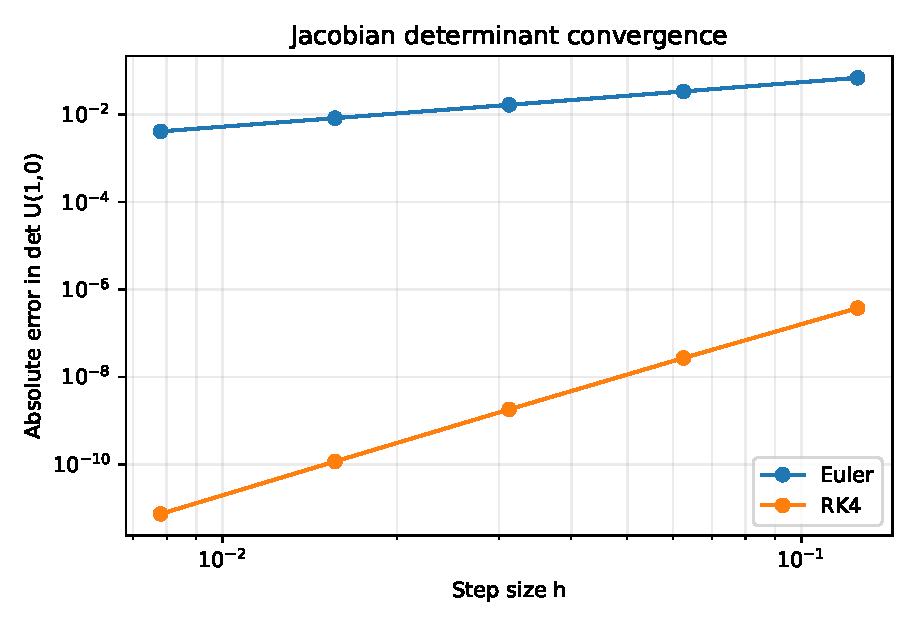
\includegraphics[width=.82\linewidth]{figures/jacobian_convergence.pdf}
\caption{Log--log comparison of first-order forward Euler and fourth-order
Runge--Kutta determinant errors.}\label{fig:jacexp}
\end{figure}
The computed matrix commutator has Frobenius norm $1.32421$ and the discrepancy between the true fundamental matrix and the unordered exponential is $0.09927$. The Euler and RK4 errors in Table~\ref{tab:jacexp} exhibit the predicted orders.


\medskip\noindent\textbf{Executed numerical experiment II: identical marginals do not fix time correlations.}\par
For the coupled OU model take $(a,c,\kappa,\beta)=(0.8,1.7,1.1,1)$.
The equilibrium $X$-marginal has variance $(\beta a)^{-1}=1.25$ in
both the microscopic model and the Markov closure. The two time
correlations at lag one, however, are
\[ C_{\mathrm{full}}(1)=0.798008,\qquad C_{\mathrm{closure}}(1)=0.561661. \]

\begin{figure}[htbp]\centering
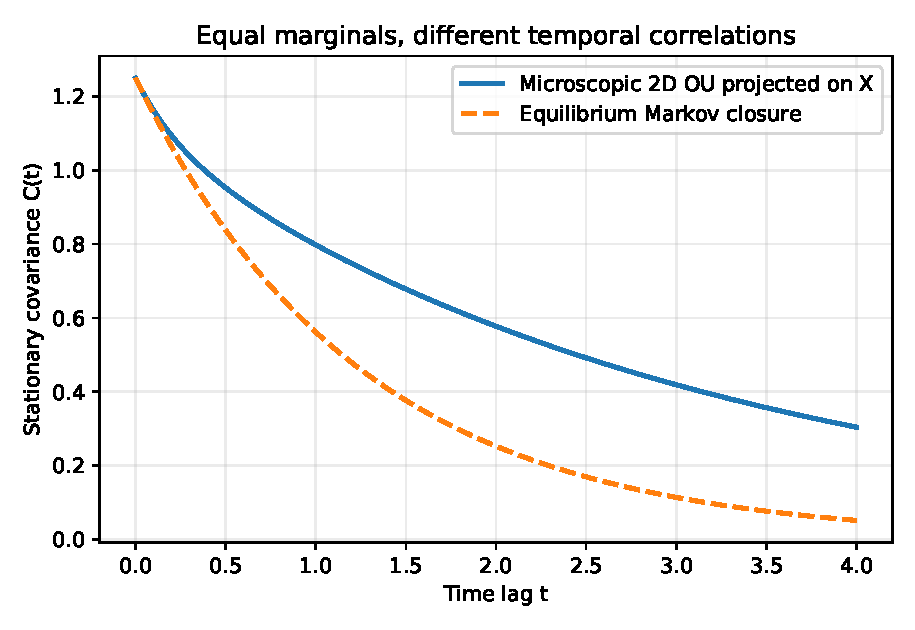
\includegraphics[width=.82\linewidth]{figures/ou_correlation.pdf}
\caption{Exact stationary two-time covariances; the curves share the same
value at zero lag but separate as soon as their temporal dynamics matters.}
\label{fig:ou-correlation}
\end{figure}

\medskip\noindent\textbf{Executed AI experiment: learning a projected drift.}\par
With the same model and nonstationary Gaussian initial data
$m_0=(1,-0.8)^\top$, $\Sigma_0=\operatorname{diag}(0.12,0.25)$,
we sampled the exact Gaussian law at times $t\in\{0.25,0.5,1,2\}$.
The regression input is $(t,X_t)$, its noisy label is $Y_t$, and the
population target is the conditional mean
$g_t(x)=\E[Y_t\mid X_t=x]$ from \eqref{eq:ouconditional}. A two-hidden-layer
Tanh network with 48 units per layer is fit by Adam with fixed seed
\texttt{20261102}. We also fit a separate affine least-squares model at
each training time; the latter incorporates the Gaussian conditional
structure and is a meaningful physics-informed baseline. All errors are
measured on 12,000 independently generated test samples against the
\emph{exact conditional mean}, rather than against the noisy response.

\begin{table}[htbp]\centering\small
\caption{Held-out RMSE in the learned conditional mean $g_t(x)$.
The projected-drift RMSE equals $c|\kappa|$ times these values.}
\label{tab:ml-benchmark}
\begin{tabular}{@{}rrr@{}}\toprule
Training pairs & Neural network & Affine Gaussian baseline\\\midrule
512 & 0.07427 & 0.07414 \\
4096 & 0.09911 & 0.03552 \\
\bottomrule\end{tabular}\end{table}
\begin{figure}[htbp]\centering
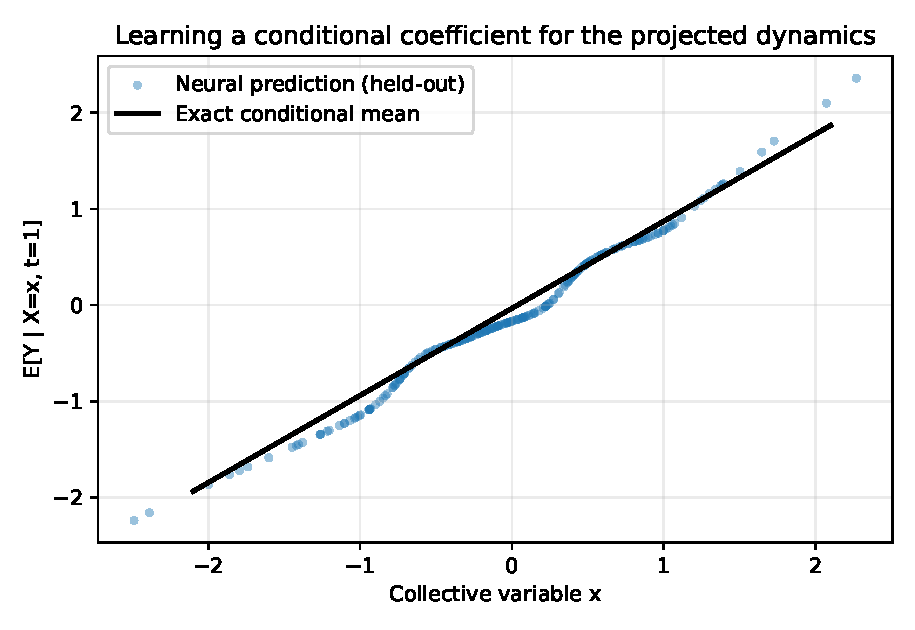
\includegraphics[width=.82\linewidth]{figures/conditional_regression.pdf}
\caption{Neural conditional-mean predictions on held-out samples at $t=1$
compared with the exact Gaussian regression function.}
\label{fig:ml-benchmark}
\end{figure}

The model is a regression surrogate for a drift coefficient; it does not
by itself demonstrate correct long-time trajectories. In this one-seed
experiment the larger training set improves the structure-aware affine
baseline, while the unconstrained neural network does not improve
monotonically. This distinction is part of the result, not a convergence
claim from two sample sizes. The exact Gaussian formulas provide an
unambiguous ground truth for later training-size and architecture studies.

\medskip\noindent\textbf{Executed Markov semidiscretization check.}\par
On $[0,1]$, use $D=1/2$, $V(x)=2(x-0.3)^2+0.7x$, and 60 finite-volume
cells. The continuous-time generator from \eqref{eq:markovrates} is
propagated by a matrix-exponential action; time is not discretized.
The initial cell-mass vector is proportional to
$\exp[-((x_i-.75)/.11)^2]$. Total mass, minimum cell mass, and
discrete relative entropy verify the relevant analytic invariants:
\begin{table}[htbp]\centering\small
\caption{Computed conservation, positivity, and equilibrium relative entropy.}
\label{tab:markov-validation}
\begin{tabular}{@{}rrr@{}}\toprule
$t$ & $\min_i m_i(t)$ & $\KL(m_t\Vert\pi)$\\\midrule
0.000 & 1.5453e-21 & 2.144403 \\
0.015 & 2.6201e-07 & 1.472250 \\
0.050 & 7.0263e-04 & 0.826780 \\
0.200 & 3.4791e-03 & 0.077412 \\
0.500 & 1.6399e-03 & 0.000610 \\
\bottomrule\end{tabular}\end{table}
The largest absolute mass discrepancy in these reported time points is
below $2\times10^{-13}$, consistent with roundoff. Entropy decreases,
as required by the exact semidiscrete dissipation identity
\eqref{eq:discreteent}.

\begin{Notice}[Reproducible experiments]
Run \texttt{python experiments/run\_benchmarks.py} after installing
\texttt{numpy}, \texttt{scipy}, \texttt{matplotlib}, and \texttt{torch}.
The script writes the PDF figures and CSV/JSON tables used above.
The seed, matrix parameters, initial laws, optimization settings, and
reference formulas are contained in the source file.
\end{Notice}

\medskip\noindent\textbf{Source mapping and corrected identities.}\par
The completed chapter incorporates Project~9 questions 1--15 as
mathematical results, worked variational calculations, or explicit
problem formulations where the original terminal functional is
unspecified. Project~10 questions 1--4 form the Hamiltonian application.
Selected results from Projects~11, 12, 13, and 14 enter the same
progression, while the continuous-time Markov discretization and its
analyzed centered alternative originate in Project~8. Two source statements require
careful correction: a noncommuting time-dependent Jacobian is
\emph{not} given by an ordinary exponential, and the KL-rate sign in
Project~9--12 is positive for the continuity convention used here.
The physical and AI exercises are placed adjacent to their models.

\medskip\noindent\textbf{Reproducibility and interpretation.}\par
The reproducibility material delivered with this chapter consists of
\path{experiments/run_benchmarks.py}, its tabular output, and three
figures. It tests the matrix ODE, the OU model, conditional regression,
and a probability-preserving spatial approximation. All finite sample
statistics are explicitly labeled as empirical, while the theorems do
not depend on them. The proposed nonlinear double-well study remains a
research exercise, not an executed experiment.


\paragraph{Detailed map to the selected source exercises.}
The source for every entry in the table is the original
\emph{Student Assessment Exercise} portfolio \cite{assessment}.
The source item numbers are preserved exactly, even though proofs and
applications have been reorganized to follow a mathematical progression.
The mapping below records the role of each selected problem in the
chapter. ``Conditional'' means the source claim has been proved under
explicit mathematical hypotheses, not that the computational result
has been assumed in advance. The nonlinear double-well extension is a
research problem, not an unreported experiment.
\begin{longtable}{@{}p{21mm}p{57mm}p{67mm}@{}}
\caption{Assessment-to-chapter map: mathematical role and location.}
\label{tab:source-map}\\
\toprule
Source & Main mathematical object & Final disposition\\\midrule\endfirsthead
\toprule Source & Main mathematical object & Final disposition\\\midrule\endhead
9.1 & Affine ODE and variation of constants & Section~\ref{ch:foundations}: complete worked derivation and matrix theorem\\
9.2 & Composition, inverse, reversal & Section~\ref{ch:foundations}: flow theorem and proof\\
9.3 & Variational matrix equation & Section~\ref{ch:foundations}: corrected noncommutative result\\
9.4 & Jacobian and numerical convergence & Section~\ref{ch:foundations}: theorem and discrete error derivation; Section~\ref{ch:benchmark}: experiment\\
9.5 & Volume of a transported domain & Section~\ref{ch:foundations}: corollary and change-of-variable proof\\
9.6 & Minimum-action path & Section~\ref{ch:foundations}: Cauchy--Schwarz solution and nonuniqueness discussion\\
9.7--9.9 & Continuity, density transport, material derivative & Section~\ref{ch:foundations}: three proofs\\
9.10--9.12 & Entropy, score, Hessian, KL-rate & Section~\ref{ch:entropy}: theorem, corollary, and sign check\\
9.13 & First variation of transported KL & Section~\ref{ch:learnedflows}: Eulerian and Lagrangian variations\\
9.14 & Constructing a target transport & Section~\ref{ch:learnedflows}: quantile construction and sample-only limits\\
9.15 & Kinetic optimal control & Section~\ref{ch:learnedflows}: formal stationarity system for specified terminal energy\\
10.1--10.4 & Hamiltonian equations, conserved energy, time reversal, symplecticity & Section~\ref{sec:hamiltonian-application}: proofs, oscillator and experiment\\
11.1, 11.5--11.8 & Gibbs inequality, Gibbs/DV duality, KL chain rule, Stein identity & Section~\ref{ch:entropy}: rigorous results\\
12.1--12.4 & Gaussian conditional law, noisy levels, coarea, mean force & Section~\ref{ch:coarsegraining}: explicit calculations and theorems\\
13.1--13.3 & Variance, It\^o projection, mimicking of marginals & Section~\ref{ch:effective}: proofs and qualified Markov projection\\
14.1--14.3 & Gaussian interpolants, conditional velocity, conditional score & Section~\ref{ch:learnedflows}: exact formulas and proofs\\
8, main and item 1 & Positivity-preserving Markov discretization; limitations of centered scheme & Section~\ref{ch:numerical}: generator theorem, entropy dissipation, code\\
\bottomrule
\end{longtable}

\paragraph{What is deliberately not claimed.}
The present chapter proves the selected results above and reports
executed deterministic, stochastic, and regression benchmarks. It does
not purport to solve every project in the broader 33-page assessment
portfolio, nor does it claim exact finite-data recovery of arbitrary
probability flows. In Project~9.15 the terminal functional must be
specified to determine an optimizer. In Project~13.3 equality of
marginals is conditional on well-posedness of the forward equation;
it does not establish equality of path laws.



\clearpage
\chapter*{Source Index and Direct Links}
\addcontentsline{toc}{chapter}{Source Index and Direct Links}
\markboth{Source Index and Direct Links}{Source Index and Direct Links}
\phantomsection\label{ch:source-index}
Each blue project entry below links directly to the corresponding theorem,
proposition, derivation, application, or solved exercise. The page number is
also a clickable link to that location. Project and question numbers refer
to the \emph{original assessment PDF} \cite{assessment}, not to this manuscript.
An unnumbered project task is listed as ``Main task.'' The separate entry
for Project~9, item~4 (numerics) leads to its discrete-time analysis.

\begingroup
\small
\setlength{\tabcolsep}{4pt}
\renewcommand{\arraystretch}{1.15}
\begin{longtable}{@{}p{38mm}p{14mm}p{90mm}@{}}
\toprule
\textbf{Original source} & \textbf{Page} & \textbf{Placement in the unified theory}\\
\midrule
\endfirsthead
\multicolumn{3}{@{}l}{\small\itshape Source Index and Direct Links (continued)}\\[4pt]
\toprule
\textbf{Original source} & \textbf{Page} & \textbf{Placement in the unified theory}\\
\midrule
\endhead
\bottomrule
\endfoot
\sourceindexrow{8}{Main task}{src:p8main}{Positive and mass-conserving Markov semidiscretization}
\sourceindexrow{8}{1}{src:p8q1}{Centered-difference scheme and its limitations}
\midrule
\sourceindexrow{9}{1}{src:p9q1}{Affine ODE and variation of constants}
\sourceindexrow{9}{2}{src:p9q2}{Composition, inverse, and time-reversal of flows}
\sourceindexrow{9}{3}{src:p9q3}{Variational matrix and noncommuting-matrix correction}
\sourceindexrow{9}{4}{src:p9q4}{Liouville--Jacobi determinant theorem}
\sourceindexrow{9}{4 (numerics)}{src:p9q4discrete}{Euler/RK4 Jacobian error and convergence order}
\sourceindexrow{9}{5}{src:p9q5}{Volume transport and Reynolds-type identity}
\sourceindexrow{9}{6}{src:p9q6}{Minimum-energy path and optimal velocity}
\sourceindexrow{9}{7}{src:p9q7}{Pushforward dynamics and continuity equation}
\sourceindexrow{9}{8}{src:p9q8}{Density change-of-variables formula}
\sourceindexrow{9}{9}{src:p9q9}{Material derivative and transport theorem}
\sourceindexrow{9}{10}{src:p9q10}{Differential-entropy evolution}
\sourceindexrow{9}{11}{src:p9q11}{Score evolution and Hessian extension}
\sourceindexrow{9}{12}{src:p9q12}{Relative-entropy evolution for two flows}
\sourceindexrow{9}{13}{src:p9q13}{First variation of transported KL divergence}
\sourceindexrow{9}{14}{src:p9q14}{Transport from a Gaussian to a target law}
\sourceindexrow{9}{15}{src:p9q15}{Measure-valued kinetic optimal-control problem}
\midrule
\sourceindexrow{10}{1}{src:p10q1}{Hamilton equations from the mechanical Hamiltonian}
\sourceindexrow{10}{2}{src:p10q2}{Energy conservation along trajectories}
\sourceindexrow{10}{3}{src:p10q3}{Time reversal and momentum reflection}
\sourceindexrow{10}{4}{src:p10q4}{Symplecticity and preservation of phase volume}
\midrule
\sourceindexrow{11}{1}{src:p11q1}{Nonnegativity of relative entropy}
\sourceindexrow{11}{5}{src:p11q5}{Gibbs variational identity}
\sourceindexrow{11}{6}{src:p11q6}{Donsker--Varadhan dual representation}
\sourceindexrow{11}{7}{src:p11q7}{Chain rule for relative entropy}
\sourceindexrow{11}{8}{src:p11q8}{Stein identity and its operator}
\midrule
\sourceindexrow{12}{1}{src:p12q1}{Gaussian conditional distribution}
\sourceindexrow{12}{2}{src:p12q2}{Noisy conditioning and level-set approximation}
\sourceindexrow{12}{3}{src:p12q3}{Coarea formula and effective free energy}
\sourceindexrow{12}{4}{src:p12q4}{Conditional mean-force formula}
\midrule
\sourceindexrow{13}{1}{src:p13q1}{Conditional-variance identity and reaction coordinates}
\sourceindexrow{13}{2}{src:p13q2}{It\^o equation for a collective variable}
\sourceindexrow{13}{3}{src:p13q3}{Markovian matching of time marginals}
\midrule
\sourceindexrow{14}{1}{src:p14q1}{Gaussian stochastic-interpolant statistics}
\sourceindexrow{14}{2}{src:p14q2}{Conditional interpolant velocity field}
\sourceindexrow{14}{3}{src:p14q3}{Conditional-score identity}
\end{longtable}
\endgroup

\clearpage
\printbibliography[heading=bibintoc,title={References}]
\end{document}
